\section{Continuum mechanics}

Continuum mechanics allows to define general equations of motion for a wide range of phenomena from liquids to deformable solids. In this chapter we describe the basics that allow to formulate general equations of motion, we explain the different steps that allows to numerically solve these equations and we detail the discretization for incompressible fluid using SPH and deformable solids using the frame-based model.

\begin{itemize}
\item We present a force-based framework.
\end{itemize}

\subsection{Notation}

\begin{table}[!h]
\begin{tabular}{ll}
$t$ & time \\
$m$ &  mass \\
$\rho$ & mass density \\
$\mathbf{x}$ & position \\
$\mathbf{v}$ & velocity \\
$\mathbf{f}$ & total forces \\
$\mathbf{f}_{int}$ & internal forces \\
$\mathbf{f}_{ext}$ & external forces \\
$\mathbf{F}$ & Deformation gradient \\
$\mathbf{\epsilon}$ & Strain tensor \\
$\mathbf{\sigma}$ & Stress tensor \\
$\mathbf{\Psi}$ & Energy density
\end{tabular}
\end{table}

\subsection{Equations of motion}

\subsubsection{Conservation of mass}

\begin{figure}[!ht]
\centering
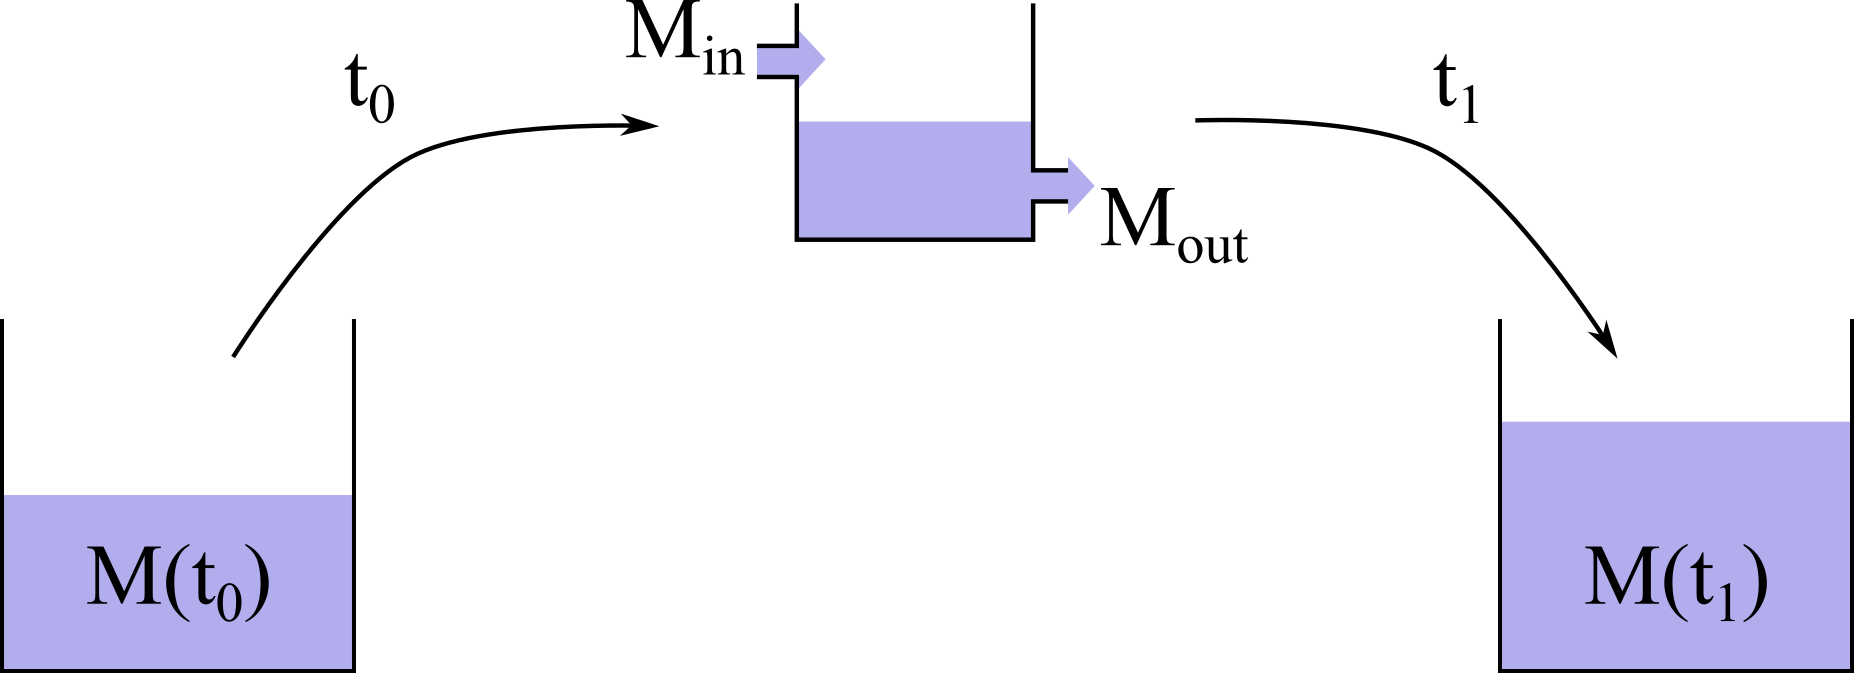
\includegraphics[scale=0.7]{images/continuum_mechanics/massConservation.png}
\caption[STAR mechanics: Mass conservation]{\label{fig:massConservation} Mass conservation. $M(t_{1}) = M(t_{0}) + M_{added} + M_{removed}$}
\end{figure}

The conservation of mass is quite explicit. Mass cannot be created or destroyed. If we look at a small volume $\mathcal{V}$ of the domain $\Omega$, the variation of mass in $\mathcal{V}$ should be equal to the flux of mass going through the border of the volume.
\begin{equation}
    \label{eq:massConservation}
    \frac{d}{dt}\left( \int_{\mathcal{V}} \rho dx \right)
    =
    - \int_{\mathcal{\partial V}}\rho \mathbf{v} \cdot \mathbf{n} ds
\end{equation}

From Stokes' formula, we have

\begin{equation}
\int_{\partial \mathcal{V}} \rho \cdot \mathbf{v} \mathbf{n} ds =
\int_{\mathcal{V}} \nabla \cdot \left( \rho \mathbf{v} \right)
\end{equation}

then the conservation of mass can be rewritten as

\begin{equation}
\int_{\mathcal{V}} \frac{d}{dt} \rho + \nabla \cdot \left( \rho  \mathbf{v} \right) dx = 0
\end{equation}

\subsubsection{Conservation of momentum}

\begin{figure}[!ht]
\centering
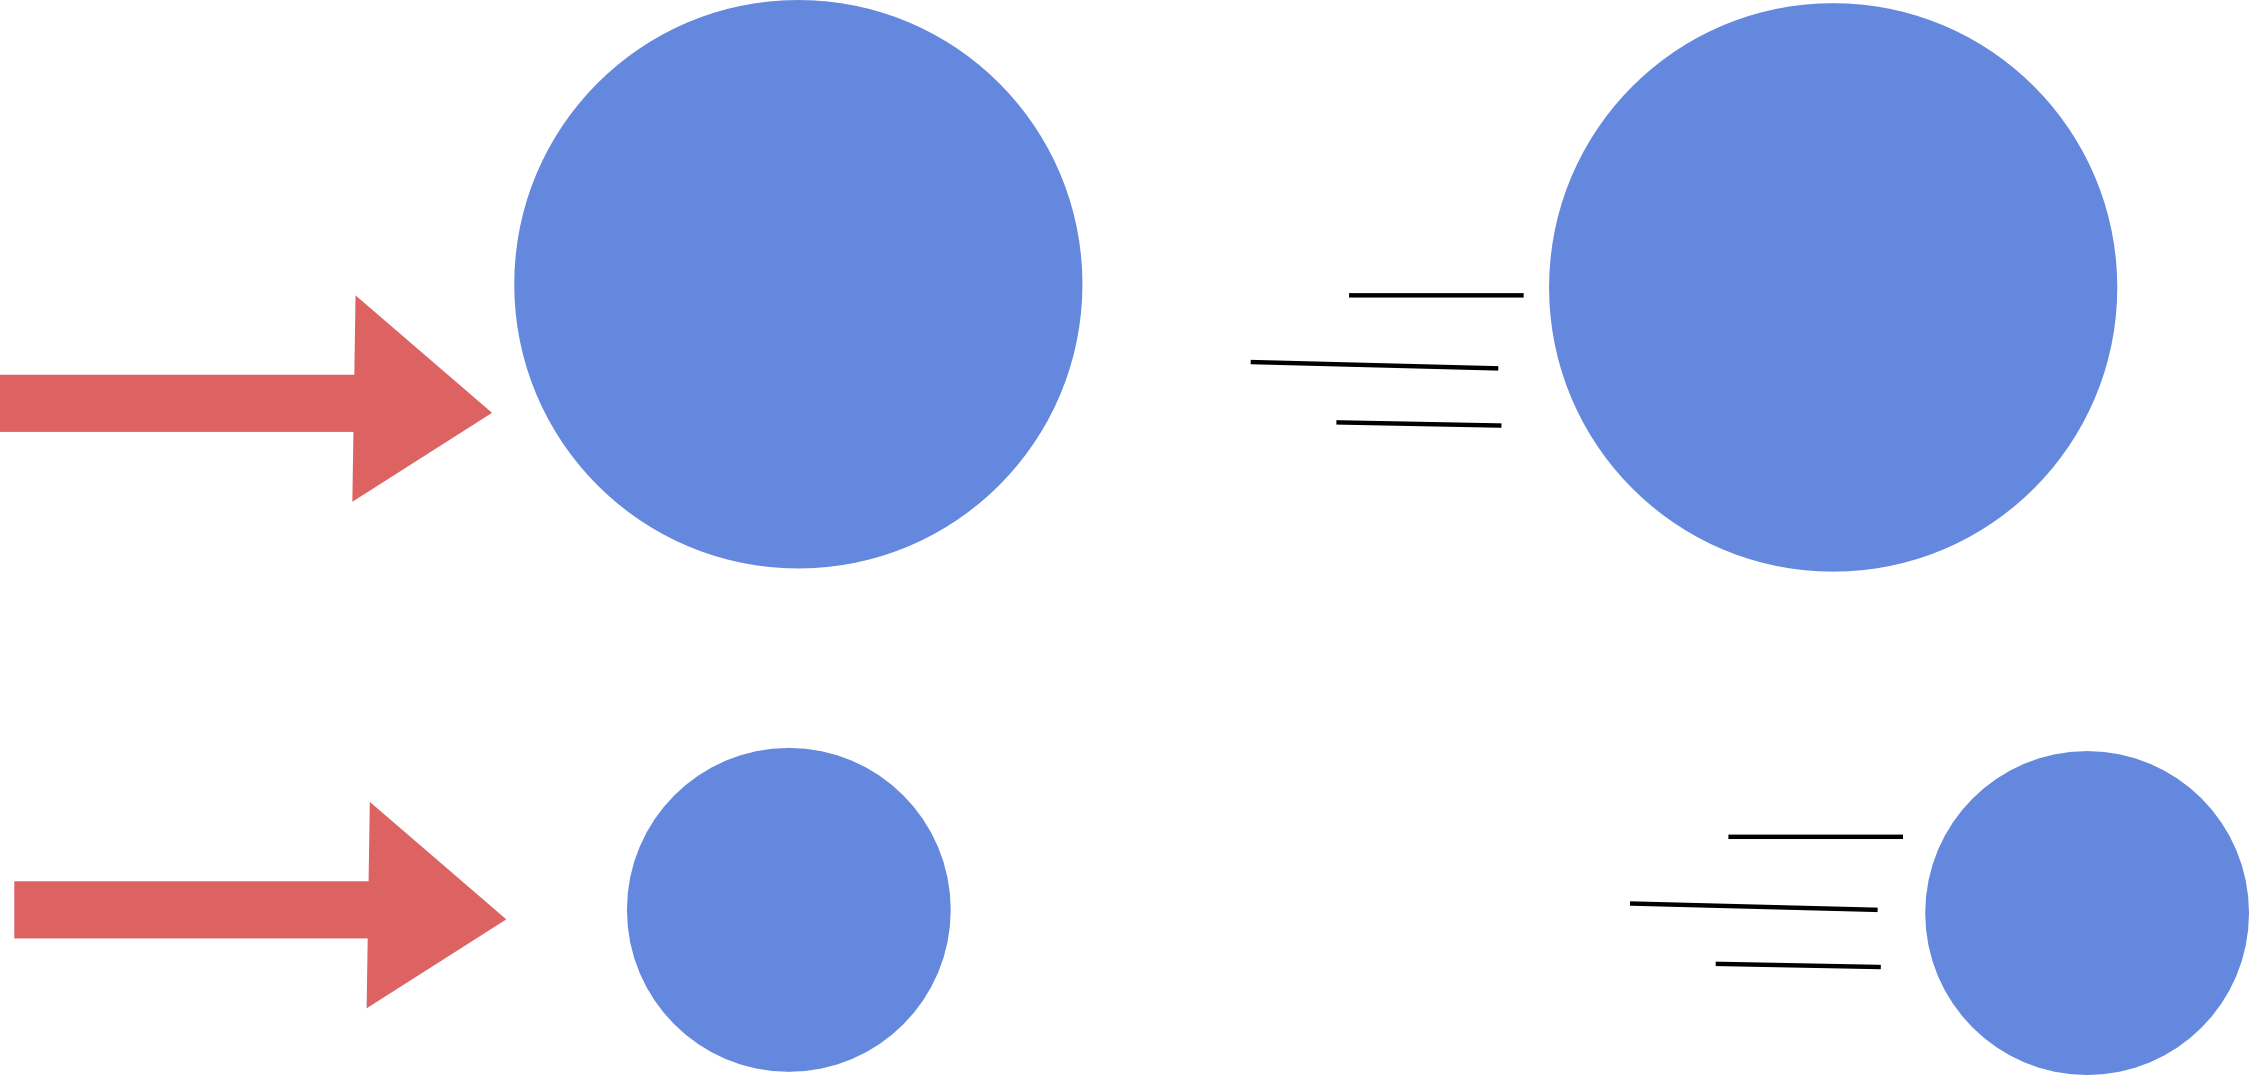
\includegraphics[scale=1.5]{images/continuum_mechanics/momentumConservation.png}
\caption[STAR mechanics: Momentum conservation]{\label{fig:momentumConservation} Momentum conservation.}
\end{figure}

Also called Newton's second law, it states:
\begin{equation}
\label{eq:momentumConservation}
\int_{\mathcal{V}} \rho \frac{D}{Dt} \mathbf{v}(t,x) dx = \int_{V} \mathbf{f} dx
\end{equation}

Two kind of forces are generally applied on an object, the \emph{external} forces and the \emph{internal} forces.

External forces describe the action of the surrounding environment on the object, the simplest example is the gravity:
\begin{equation}
\int_{\mathcal{V}} \rho \mathbf{g} dx
\end{equation}

Internal forces describe the reaction of the object to an external deformation. A general way to describe them is by using a tensor notation:
\begin{equation}
\int_{\mathcal{V}} \sigma \mathbf{n} ds
\end{equation}
By applying the Stokes' formula we can describe it with respect to the volume:
\begin{equation}
\int_{\mathcal{V}} \sigma \mathbf{n} ds =
\int_{\mathcal{V}} \nabla \cdot \sigma dx
\end{equation}

Conservation of momentum can then be rewritten:
\begin{equation}
\int_{\mathcal{V}} \rho \frac{D}{Dt} \mathbf{v}(t,x) dx = \int_{V} \rho \mathbf{g} + \nabla. \sigma dx
\end{equation}

\subsubsection{Lagrangian vs. Eulerian}

\begin{figure}[!ht]
\centering
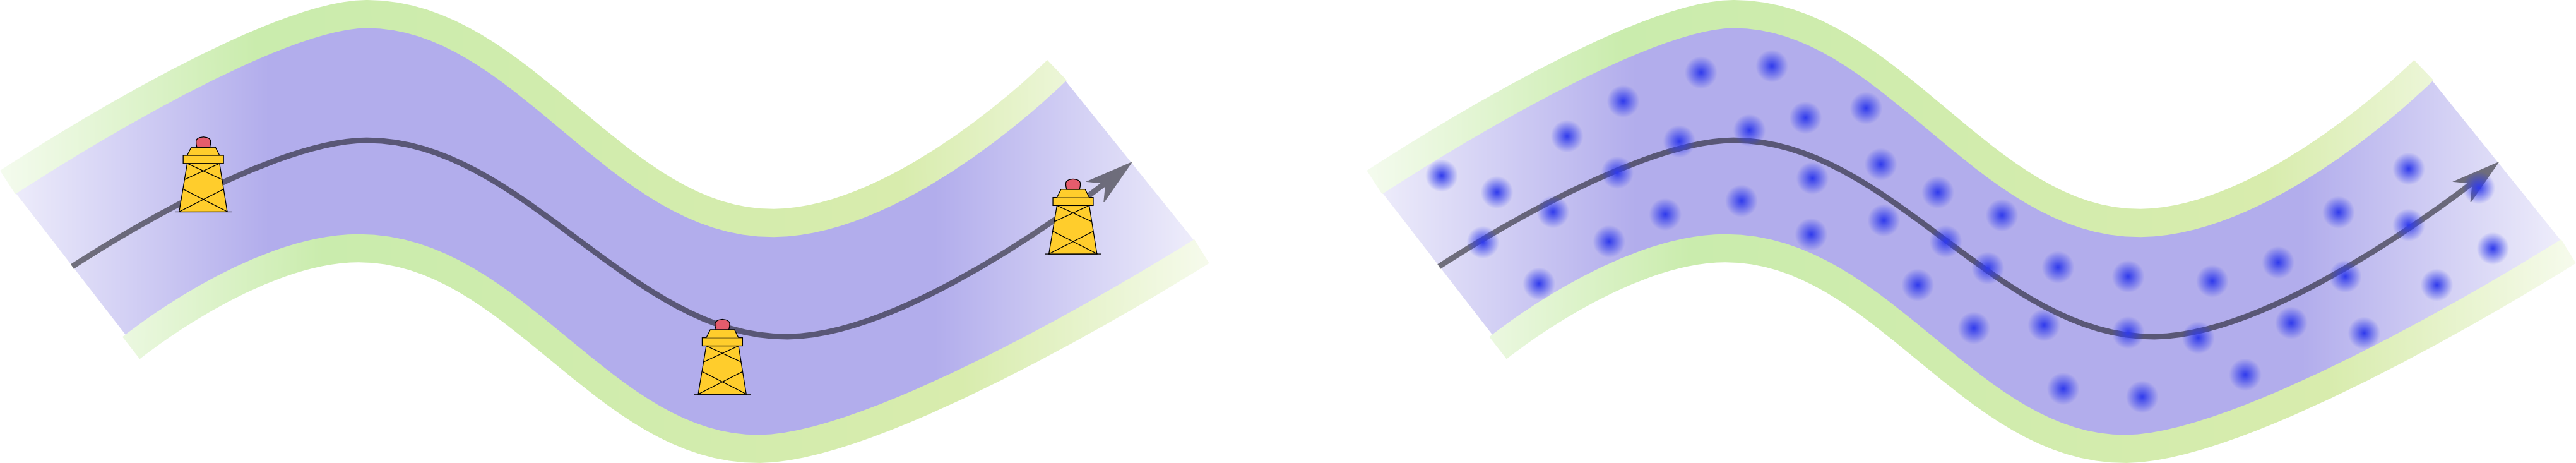
\includegraphics[scale=0.5]{images/continuum_mechanics/eulerianVsLagrangian.png}
\caption[STAR mechanics: Eulerian vs. Lagrangian]{\label{fig:eulerianVsLagrangian} Eulerian vs. Lagrangian viewpoint}
\end{figure}

Lagrangian: You follow the river. The river is discretized into particles which carries and update fluid properties such as position and velocity. 

Eulerian : You stand in the middle of a river. The river is discretized into a fixed grid from where you can measure the velocity of the flow passing through the point of the grid.

The material derivative:
\begin{equation}
\frac{D\mathbf{u}}{Dt} = \frac{\partial \mathbf{u}}{\partial t} + (\mathbf{u} \cdot \nabla v)
\end{equation}

In a lagrangian framework, the positions of the particles at a specific time $t$ is known, so the material derivative is just the time derivative.

\begin{equation}
\frac{D\mathbf{u}}{Dt} = \frac{\partial u}{\partial t}
\end{equation}

Moreover, if we assume that the mass of the particles is constant through the simulation, then conservation of mass is granted and we can omit its numerical solving. However, in practice it does not ensure that the divergence of the velocity will be null, new methods were proposed to enforce the null divergence condition. In this work we keep the first approximation and do not enforce the null divergence condition.

\subsubsection{Numerical solving}

Once the equations of motion are stated, they are discretized in space an time in order to be numerically solved.

\paragraph{Spatial discretization}

\begin{figure}[!ht]
\centering
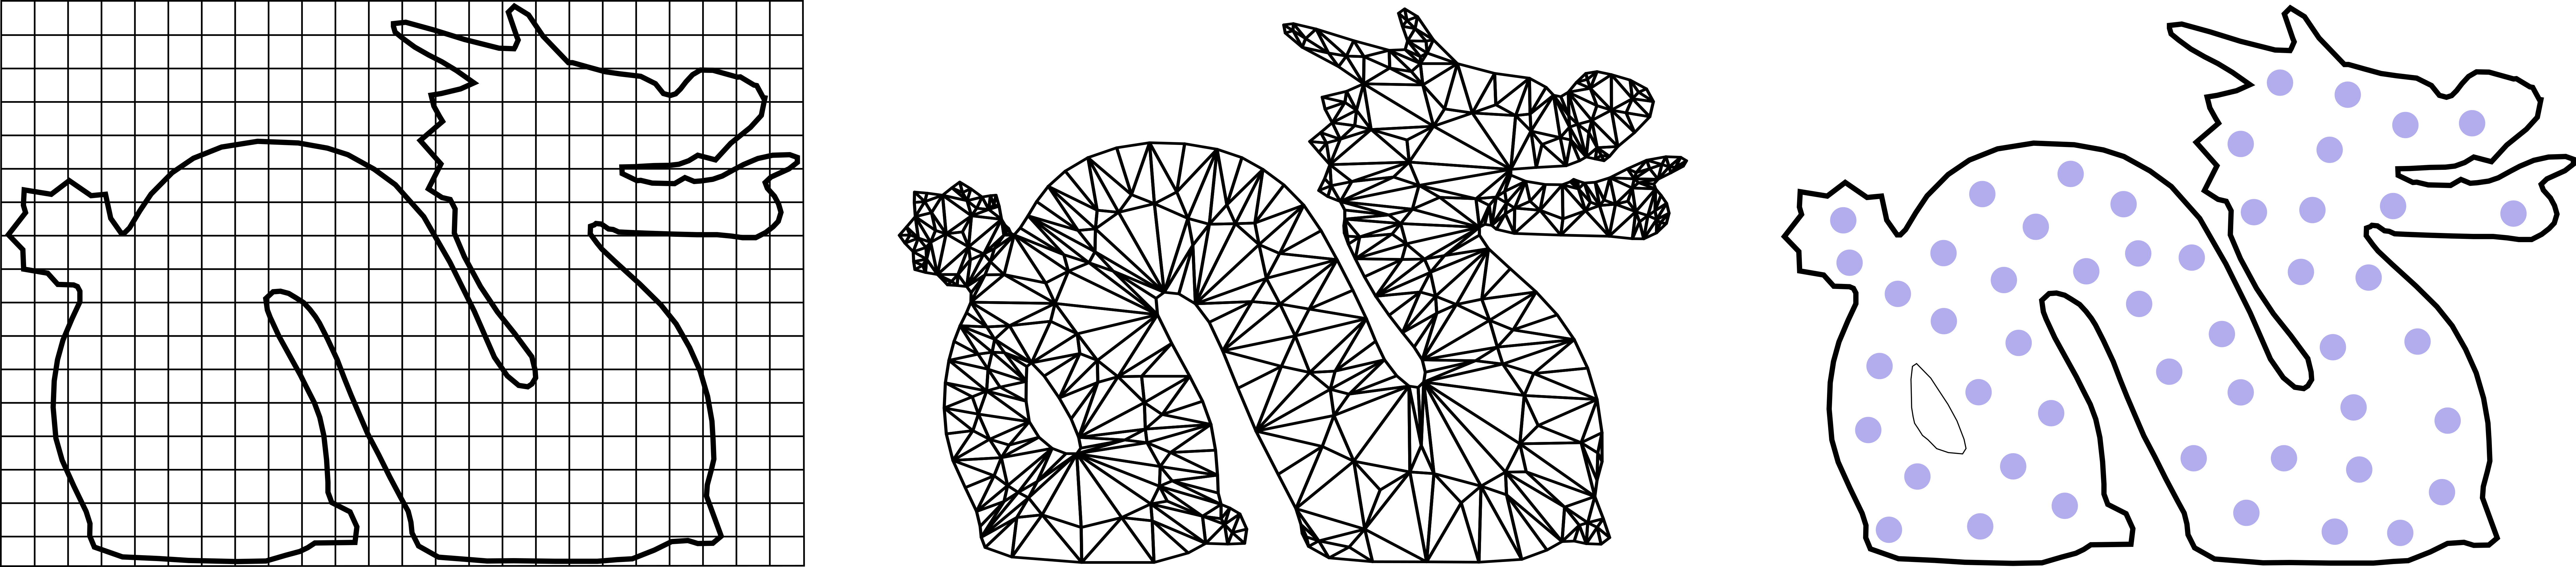
\includegraphics[scale=0.2]{images/continuum_mechanics/discretization.png}
\caption[STAR mechanics: Discretization]{\label{fig:discretization} Three kind of discretization.}
\end{figure}

The spatial discretization consists in approximating the object to simulate with a finite number of samples called the degrees of freedom. Then by using an interpolation method, it is possible to approximate the continuous quantity, such as position, velocity, density and so on, over all the domain. Finally, a quadrature rule is needed in order to integrate these quantities over the domain. These are the main components for solving the equations of motion:
degrees of freedom, an interpolation method, a quadrature rule. 

Multiple possibilities exists for these components. When choosing them, the context of the simulation needs to be taken into account.
What is the simulated phenomena ?
What do we want to measure ?
What are the restrictions in terms of computational cost and memory consumption ?
What is available in order to represent boundaries ?
Is there any topological changes occurring ?

\subparagraph{Degrees of freedom}
For Eulerian simulations, velocities are the most common degrees of freedom. Usually they are computed at fixed location regularly sampled.

For Lagrangian simulations, positions are the most common degrees of freedom. They can sample the object in many different ways depending on the interpolation method. Another possibility is to also represent orientations, this is used in the frame-based model where degrees of freedom are affine frames.

\subparagraph{Interpolation}

\begin{figure}[!ht]
\centering
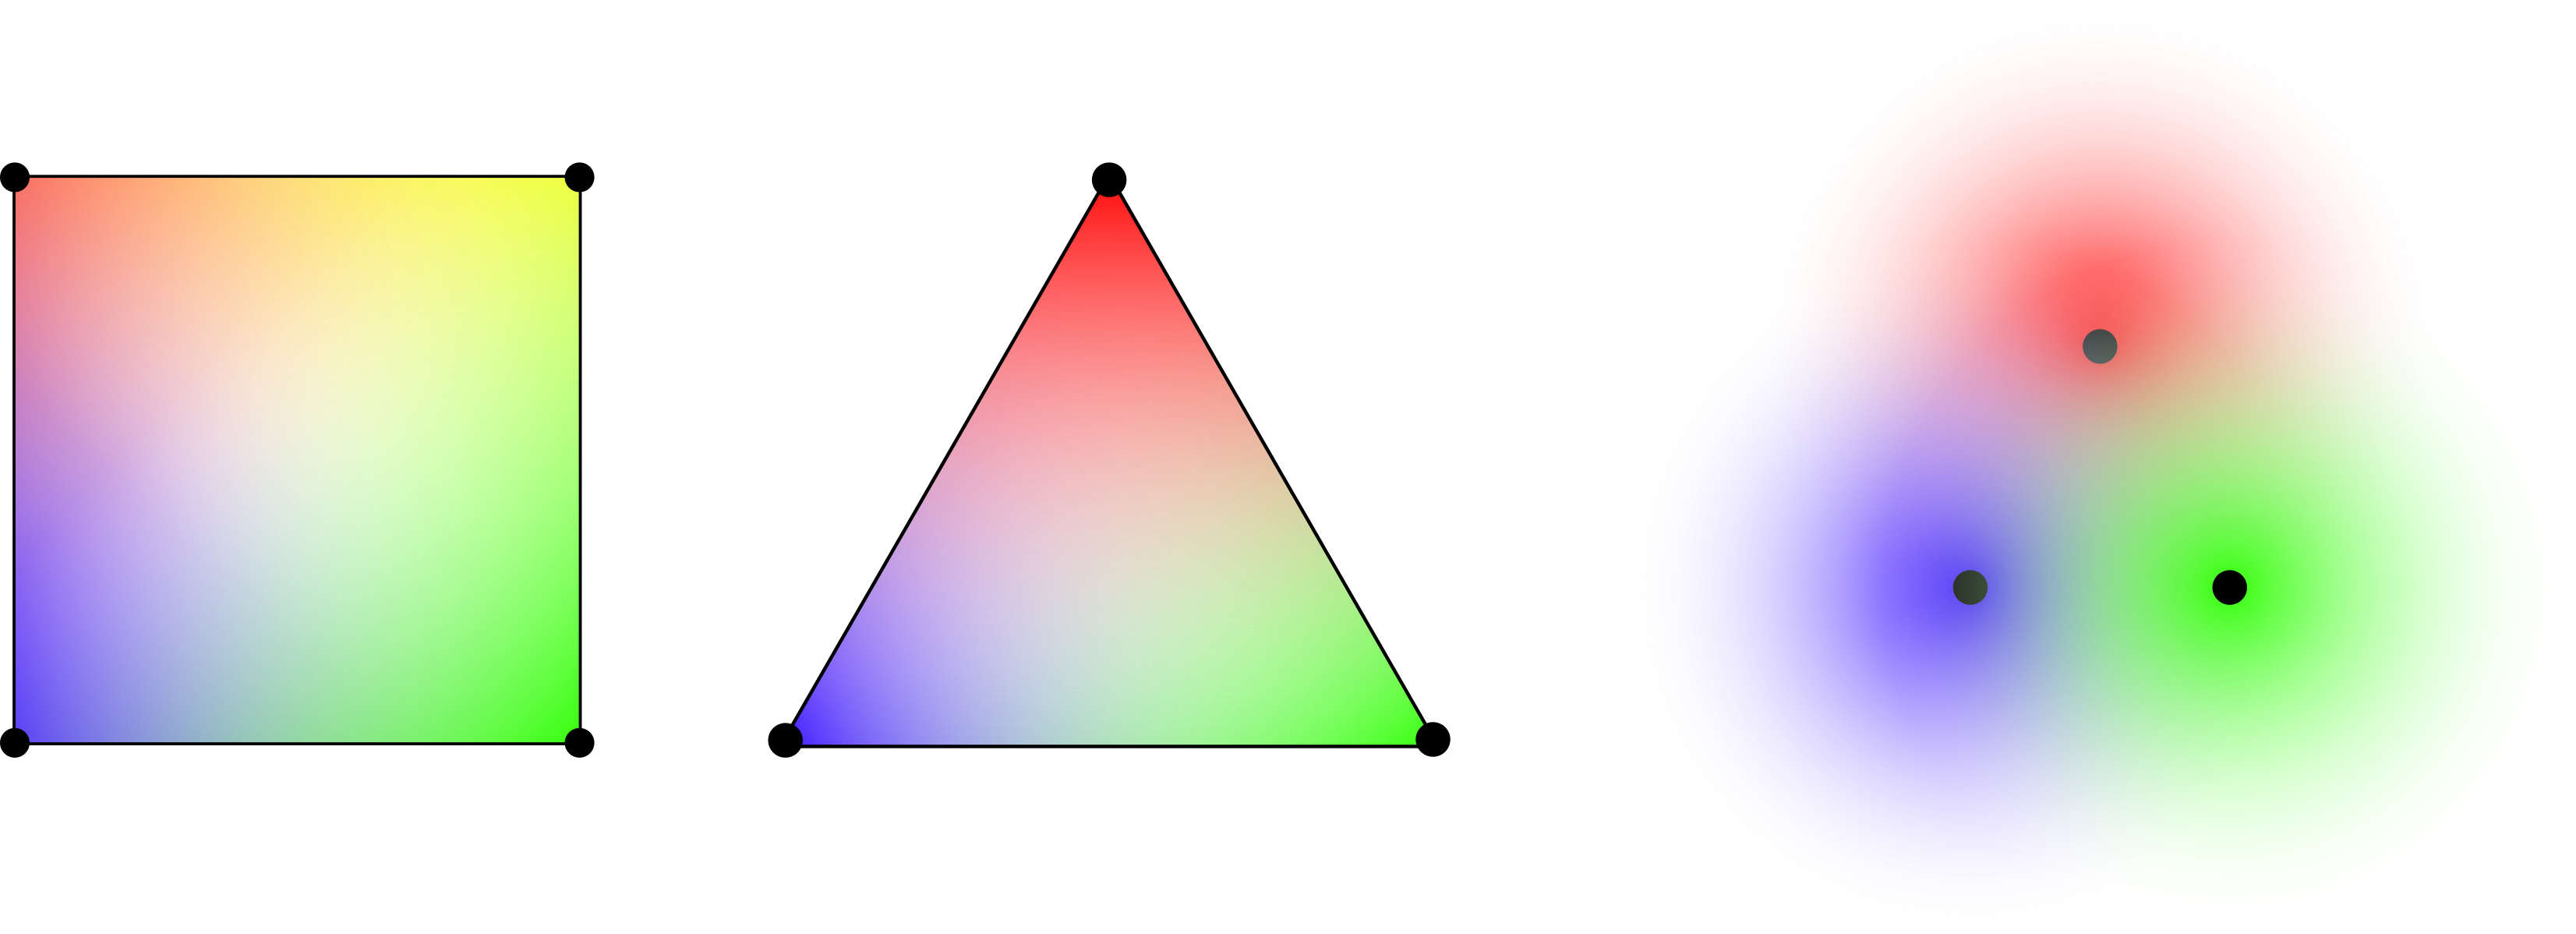
\includegraphics[scale=0.4]{images/continuum_mechanics/shapefunction.png}
\caption[STAR mechanics: Shape functions]{\label{fig:shapefunction} Example of shape functions.}
\end{figure}

In Computer Graphics, there are mainly three interpolation methods: linear interpolation, moving least squares and sph interpolation. For each of them different weights, also called shape functions can be used. 

The choice of the interpolation method and its weights changes depending on the spatial sampling of the degrees of freedom. Usually two types of sampling are distinguished: mesh-based sampling and mesh-less sampling.

In mesh-based methods, the degrees of freedom are the vertices of a mesh. Depending on its structure different possibilities exist. For grids, trilinear interpolation is often used. For unstructured meshes, linear interpolation with barycentric weights is the most popular choice.

In mesh-less methods, the sampling of degrees of freedom might be completely unstructured. For Lagrangian fluids, particles of fluid will often change of neighborhood, the structure is quasi-inexistant. For Lagrangian elastic solids, particles will keep the same neighborhood as long as the object does not undergo topological changes. The two most common interpolation methods are SPH and Moving Least Squares. Weights are often computed using cubic kernel. However if the sampling of degrees of freedom is very sparse, Voronoi-base shape functions are a good alternative.

\subparagraph{Integration}

\begin{figure}[!ht]
\centering
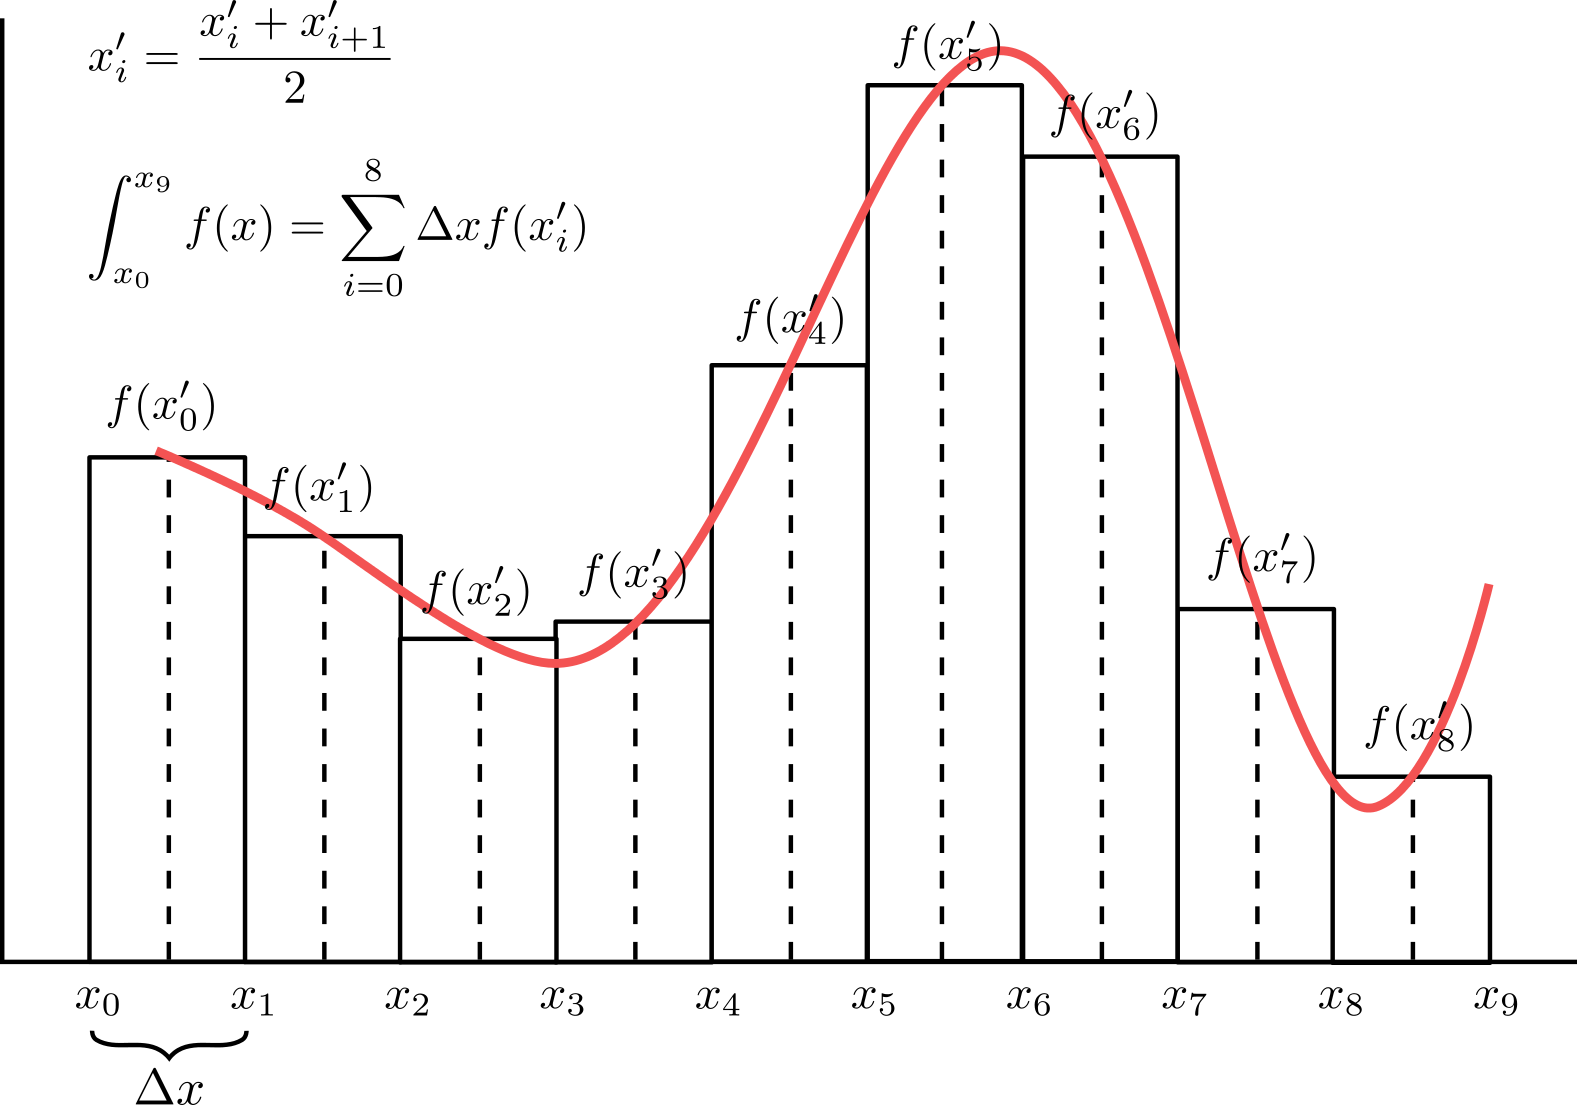
\includegraphics[scale=1.0]{images/continuum_mechanics/spatialIntegration.png}
\caption[STAR mechanics: Spatial integration]{\label{fig:spatialIntegration} Midpoint integration}
\end{figure}

A common choice in physics-based animation is to use the midpoint rule.
In mesh-based methods, one integration point is sampled at the center of each element and integrated over the volume of the element.
In mesh-less methods, when the sampling of the degrees of freedom is dense, integration points often co-located with them degrees of freedom an integrated over their associated volume. When the sampling is sparse, a dense independent sampling of integration points is used.

\paragraph{Temporal integration}

\begin{figure}[!ht]
\centering
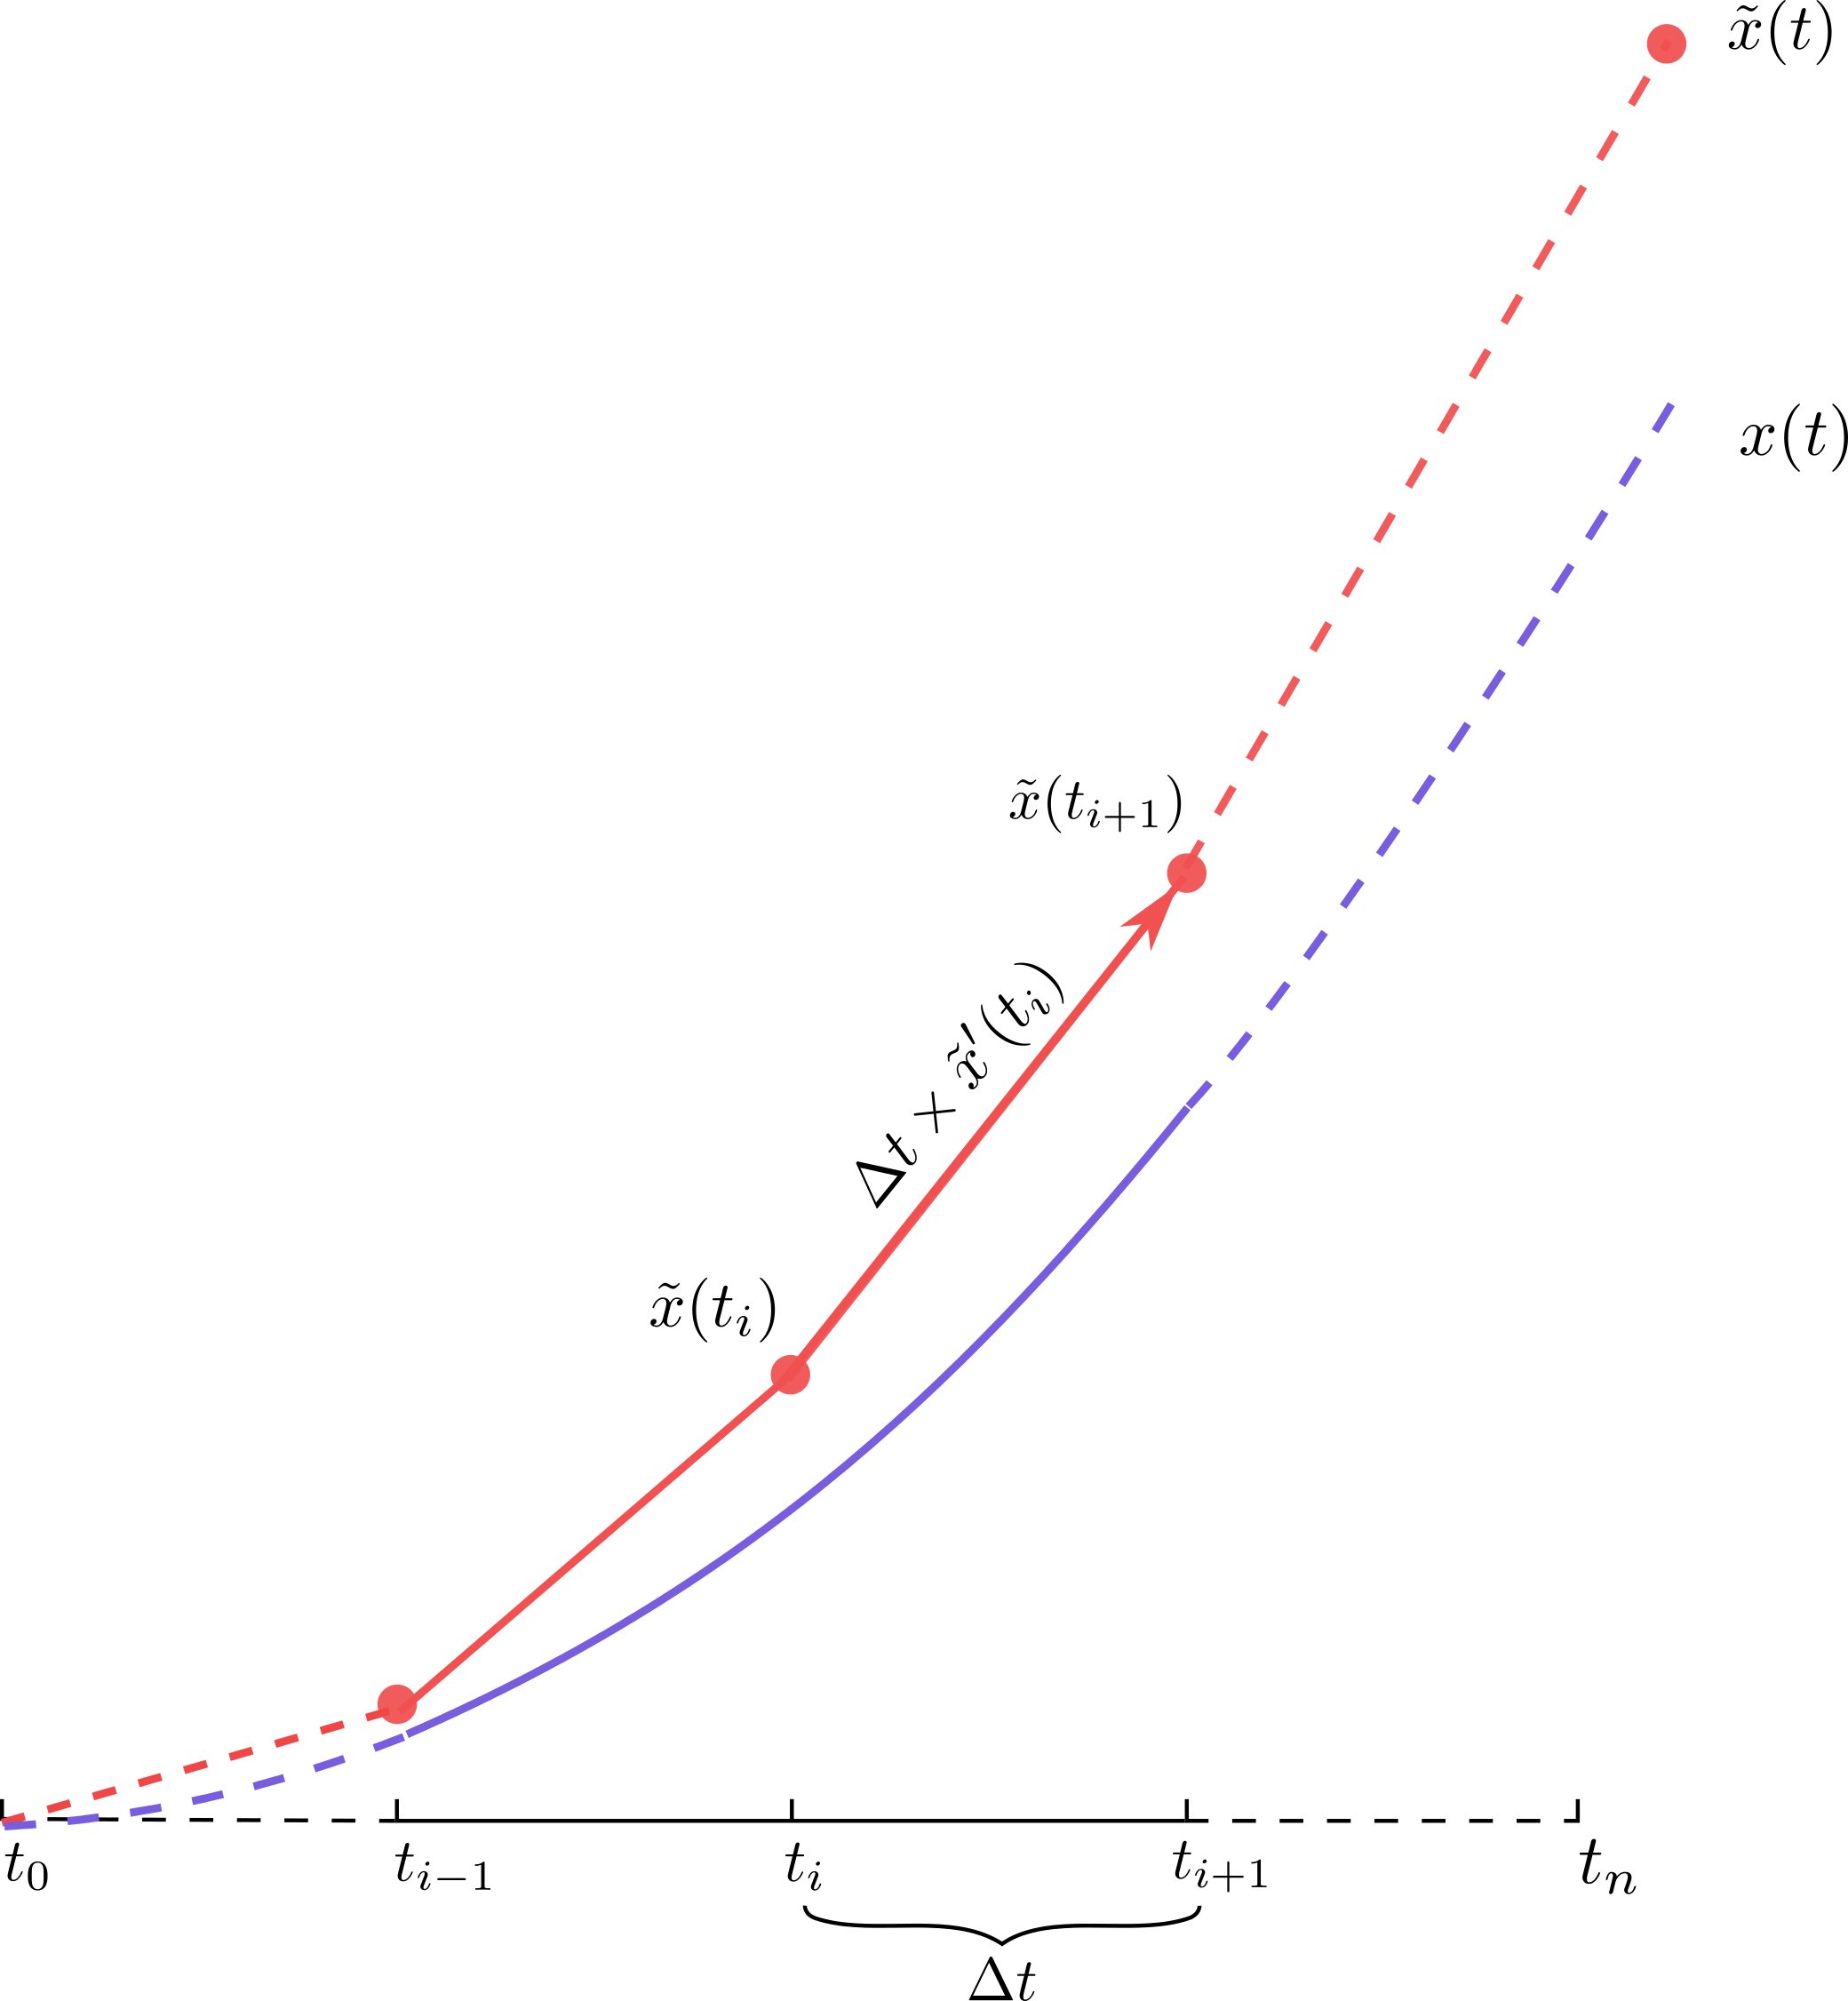
\includegraphics[scale=0.6]{images/continuum_mechanics/timeIntegration.png}
\caption[STAR mechanics: Temporal integration]{\label{fig:timeIntegration} Temporal integration}
\end{figure}

Once physical quantities have been spatially integrated, they can be integrated over time. 

\begin{equation}
\label{eq:timeIntegration1}
\displaystyle
\int_{t_{n}}^{t_{n+1}}
\rho \frac{d\mathbf{v}}{dt}
=
\int_{t_{n}}^{t_{n+1}}\mathbf{f}
\end{equation}

Many integrations scheme can be used. Most of them can be explained simply by the Taylor expansion.

\begin{equation}
\label{eq:taylorExpansion}
\displaystyle
f(x) = \sum_{k=0}^{n}\frac{\left(x-a\right)^{k}}{k!}f^{(k)}(a) + \int_{a}^{x}\frac{\left(x-t\right)^{n}}{n!}f^{(n+1)}(t)dt
\end{equation}

Applied to equation (\ref{eq:timeIntegration1}), this gives:

\begin{equation}
\label{eq:timeIntegration2}
\displaystyle
\mathbf{v}(t_{n+1}) = \mathbf{v}(t_{n}) + \int_{t_{n}}^{t_{n+1}}\frac{1}{\rho}\frac{d\mathbf{v}}{dt}
\end{equation}

The expression can be further expanded in order to get more accurate result. In Computer Graphics, this is the most used expansion. Generally, the integral term is computed with the rectangle quadrature rule.

For a left rectangle method, we get an explicit integration of the velocity:
\begin{equation}
\label{eq:explicitIntegration}
\mathbf{v}(t_{n+1}) = \mathbf{v}(t_{n}) + \left(t_{n+1}-t_{n}\right) \frac{\mathbf{f}(t_{n})}{\rho}
\end{equation}

For a right rectangle method, we get an implicit integration of the velocity:
\begin{equation}
\label{eq:implicitIntegration}
\mathbf{v}(t_{n+1}) = \mathbf{v}(t_{n}) + \left(t_{n+1}-t_{n}\right) \frac{\mathbf{f}(t_{n+1})}{\rho}
\end{equation}

The same rule applies for the integration of other physical quantities. In a Lagrangian system, velocity and position both needs to be integrated. In general, three different schemes are used: forward Euler, symplectic Euler and backward Euler.

Forward euler is the explicit integration of both position and velocity:
\begin{equation}
\label{eq:explicitEuler}
\begin{array}{l}
\displaystyle x(t+\Delta t) = x(t) + \Delta t \mathbf{v}(t) \\ \\
\displaystyle v(t+\Delta t) = v(t) + \Delta t \frac{\mathbf{f(t)}}{\rho}(t)
\end{array}
\end{equation}

Symplectic euler is the explicit integration of velocity and implicit integration of position:
\begin{equation}
\label{eq:symplecticEuler}
\begin{array}{l}
\displaystyle v(t+\Delta t) = v(t) + \Delta t \frac{\mathbf{f}(t)}{\rho} \\ \\
\displaystyle x(t+\Delta t) = x(t) + \Delta t \mathbf{v}(t+\Delta t)
\end{array}
\end{equation}

Backward euler is the implicit integration of both position and velocity
\begin{equation}
\label{eq:backwardEuler}
\begin{array}{ll}
\displaystyle v(t+\Delta t) = v(t) + \Delta t \frac{\mathbf{f}(t)}{\rho}(t+\Delta t) \\ \\
\displaystyle x(t+\Delta t) = x(t) + \Delta t \mathbf{v}(t+\Delta t)
\end{array}
\end{equation}

Forward and symplectic Euler are among the easiest integration scheme. They are easy cheap and easy to implement. However stability is guaranteed for a restricted range of time steps. Implicit euler is more expensive as it results in solving an equation. However unconditional stability is guaranteed which means that large time steps can be used resulting in a significant speed-up of the simulation. 

A nice way to solve the equation of backward Euler is to expand the force expression in order to fall back to solving a linear system. There, efficient iterative methods such as the conjugate gradient can be used.

\subsection{Fluid mechanics}

\subsubsection{Constitutive Law}

Fluid may be subject to an additional constraint whether they are incompressible or not. Incompressibility states that the mass should not vary over time. Then the mass conservation can be rewritten as:
\begin{equation}
\nabla \cdot \mathbf{v} = 0
\end{equation}

For an incompressible fluid, the fluid reacts to pressure and viscosity and thus the constitutive law can be written as:
\begin{equation}
\sigma = -pI + \eta \left( \nabla \mathbf{v} + \nabla \mathbf{v}^{T} \right)
\end{equation}

Then we have:
\begin{equation}
\nabla \cdot \sigma = \nabla \cdot \left( -pI + \eta \left( \nabla \mathbf{v} + \nabla \mathbf{v}^{T} \right) \right) = -\nabla p + \Delta \mathbf{v}
\end{equation}

With internal forces, we have the Navier-Stokes equation for an incompressible fluid:

\begin{equation}
\begin{array}{ll}
\displaystyle
\int_{\mathcal{V}} \rho \frac{D}{Dt} \mathbf{v}(t,x) dx = \int_{V} \rho \mathbf{g} -\nabla p + \eta \Delta \mathbf{v} dx \\ \\
\displaystyle
\nabla. \mathbf{v} = 0
\end{array}
\end{equation}

\subsubsection{SPH model}
Smoothed Particles Hydrodynamics is an interpolation method that can be used to discretize the Navier-Stokes equation in a Lagrangian way. The fluid is discretized into particles which represent a small volume of the whole fluid and each quantity is interpolated using SPH.

\paragraph{SPH interpolation}
The interpolation of a function $f$ at a position $\mathbf{x}$ is :
\begin{equation}
f(\mathbf{x}) = \int_{V} f(\mathbf{x'})W(\mathbf{x}-\mathbf{x'}, h)dx'
\end{equation}
where $W$ is a function called \emph{kernel}. 

If the fluid is discretized into particles with a mass $m$, a density $\rho$ and a volume $V$, then we can discretize the SPH interpolation as:
\begin{equation}
f(\mathbf{x}) = \sum_{p} f(\mathbf{x}_{p})V_{p} W(\mathbf{x}-\mathbf{x_{p}},h) = \sum_{p} f(\mathbf{x}_{p})\frac{m_{p}}{\rho_{p}} W(\mathbf{x}-\mathbf{x_{p}},h)
\end{equation}

Then derivatives can be computed and discretized the same way:
\begin{equation}
D^{\alpha} f(\mathbf{x}) = \int_{\mathcal{V}} f(\mathbf{x'}) D^{\alpha} W(\mathbf{x}-\mathbf{x'}, h)dx'
\end{equation}

\begin{equation}
D^{\alpha} f(\mathbf{x})= \sum_{p} f(\mathbf{x}_{p})\frac{m_{p}}{\rho_{p}} D^{\alpha} W(\mathbf{x}-\mathbf{x_{p}},h)
\end{equation}

However, for first derivatives, the approximation does not vanish if $f$ is constant. A quick way to ensure that is to use a differentiable function $\Phi$ (in practice we use the density $\rho$) to re-write the derivative using the derivative of a product :
\begin{equation}
\nabla f(x) = \frac{1}{\Phi}\left(\nabla (f \Phi) - f \nabla \Phi \right)
\end{equation}

\paragraph{How to choose the kernel}
The properties of $W$ can vary with respect to the properties of the function to be interpolated. In general, $W$ meet the following properties:
\begin{itemize}
\item $W$ is normalized. Thus, constants are interpolated exactly.
\item $W$ has a compact support.
\begin{equation}
\parallel \mathbf{x} \parallel \geq h \rightarrow W(\mathbf{x},h) = 0 
\end{equation}
\begin{equation}
\int_{\mathcal{V}} W(\mathbf{x},h) dx = 1
\end{equation}
\item $W$ tend to the delta function when the length scale $h$ tends to $0$.
\begin{equation}
\lim_{h \rightarrow 0} W(x,h) = \delta(x)
\end{equation}
\item $W$ should be symmetric to enforce invariance under rotation
\begin{equation}
W(-x,h) = W(x,h)
\end{equation}
\item Depending on the function to interpolate the kernel should be positive to prevent unphysical interpolated value.
\begin{equation}
W \geq 0
\end{equation}
\end{itemize}

The cubic kernel from Monaghan is a good choice in practice.

\paragraph{Applications to Navier-Stokes}

\begin{equation}
\rho_{i} = \sum_{j} m_{j}W(\mathbf{x_{i}}-\mathbf{x_{j}},h)
\end{equation}

\begin{equation}
\left(\nabla p\right)_{i} = \sum_{j} \frac{m_{j}}{\rho_{j}} p_{j} \nabla W(\mathbf{x_{i}}-\mathbf{x_{j}},h)
\end{equation}

However linear and angular momentum are not conserved as the formula is not symmetric. By using the previous technique with $\Phi = \frac{1}{\rho}$, it can be symmetrized:

\begin{equation}
\left(\nabla p\right)_{i} = 
\frac{1}{\rho_{i}}
\sum_{j} m_{j} \left( \frac{p_{i}}{\rho_{i}^{2}} + \frac{p_{j}}{\rho_{j}^{2}} \right) \nabla W(\mathbf{x_{i}}-\mathbf{x_{j}},h)
\end{equation}

\begin{equation}
\left(\Delta \mathbf{v}\right)_{i} = \sum_{j} \frac{m_{j}}{\rho_{j}} \mathbf{v}_{j} \Delta W(\mathbf{x_{i}}-\mathbf{x_{j}},h)
\end{equation}

Same as for the pressure gradient, this is not symmetric. Here it can be symmetrized by using $\Phi = \rho$.

\begin{equation}
\left(\Delta \mathbf{v}\right)_{i} = \frac{1}{\rho_{i}}\sum_{j} m_{j} \left( \mathbf{v}_{j}-\mathbf{v}_{i}\right) \Delta W(\mathbf{x_{i}}-\mathbf{x_{j}},h)
\end{equation}

In practice, the evaluation of the laplacian is not accurate. Another form of viscosity based on the gradient was proposed. This is still an area of research.

\begin{equation}
\left(\Delta v\right)_{i} = 
\frac{1}{\rho_{i}}
\sum_{j} m_{j} \Pi_{ij} \nabla W(\mathbf{x_{i}}-\mathbf{x_{j}},h)
\end{equation}

where 

\begin{equation}
\Pi_{ij} = -\frac{2hc_{s}}{\rho_{i}+\rho_{j}}\frac{v_{ij}^{T}x_{ij}}{\vert x_{ij} \vert^{2} + \epsilon h^{2}}
\end{equation}

Now if we discretize Navier-Stokes for one particle $i$, we have:

\begin{equation}
m_{i}\frac{d}{dt}\mathbf{v}_{i}(t) = m_{i}\mathbf{g} - m_{i}(\nabla p)_{i} + m_{i}(\delta \mathbf{v})_{i}
\end{equation}

This equation can now be discretized in time and integrated. In practice we use the euler symplectic integrator:

\begin{equation}
\begin{array}{ll}
\displaystyle \mathbf{v}_{i}(t+\Delta t) = \mathbf{v}_{i}(t) + \Delta t \frac{d}{dt}\mathbf{v}_{i}(t) \\ \\
\displaystyle \mathbf{x}_{i}(t+\Delta t) = \mathbf{x}_{i}(t) + \Delta t \mathbf{v}_{i}(t+\Delta t)
\end{array}
\end{equation}

Several interesting implementation problems arise when dealing with particle system and more particularly particle-based fluid simulations:

\begin{itemize}
\item Boundary handling 
\item Surface reconstruction
\item Optimization (acceleration structure for spatial query)
\end{itemize}

Faire un tableau avec les références et ce que l'on peut y trouver d'intéressant.

%\paragraph{Eulerian grid}
%\paragraph{Lagrangian particles}
%\paragraph{Hybrid method}
%\paragraph{Smoothed Hydrodynamics Particles model}

\subsection{Solid mechanics}

\begin{figure}[!ht]
\centering
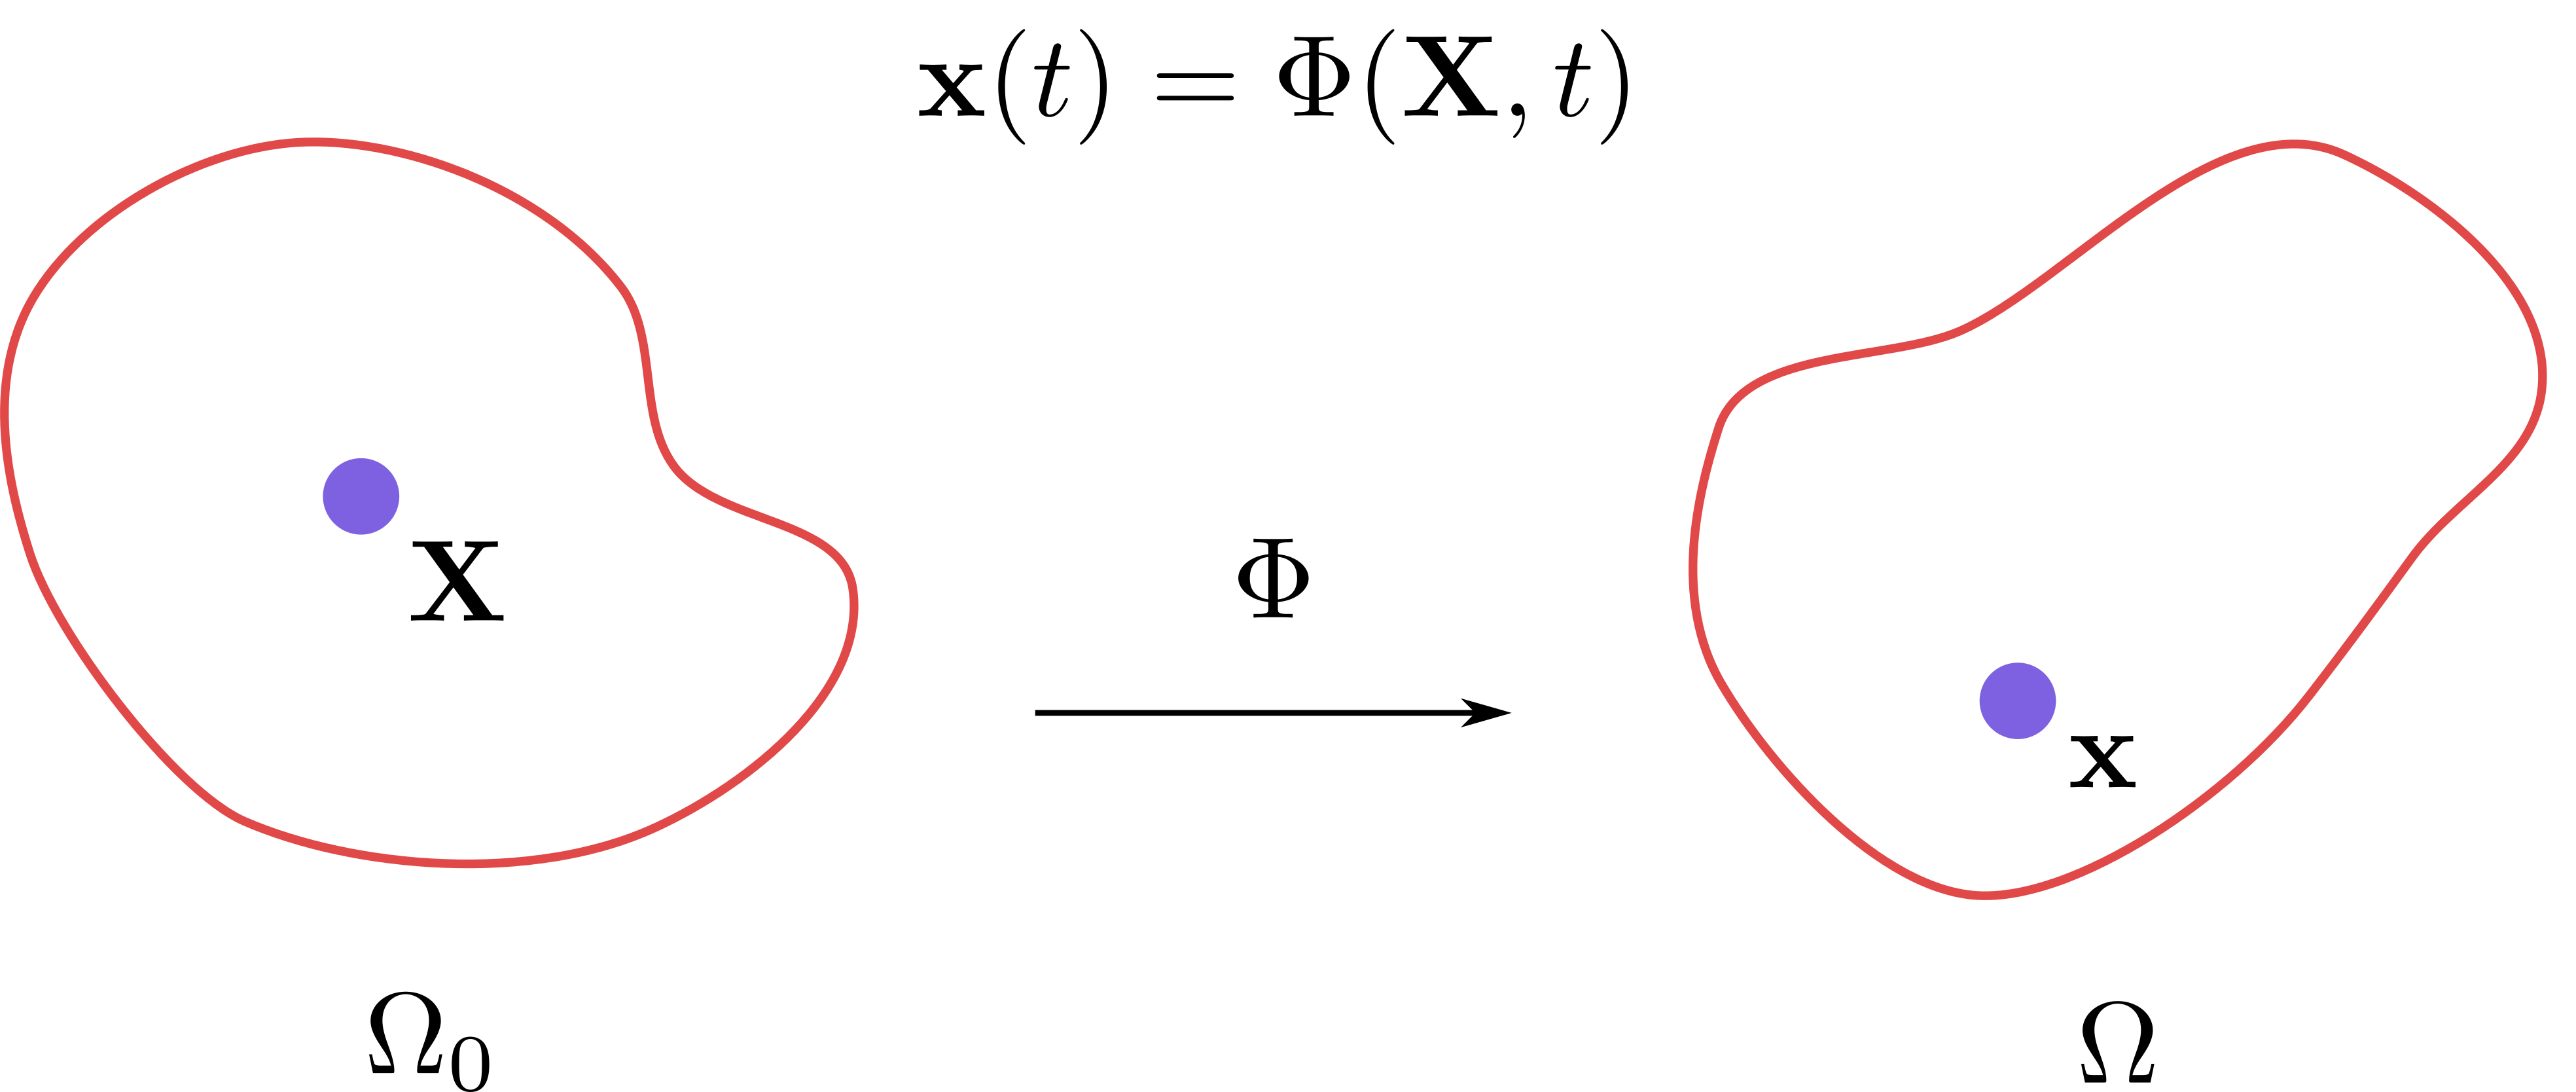
\includegraphics[scale=0.4]{./images/continuum_mechanics/displacementField.png}
\caption[STAR mechanics: Displacement field]{\label{fig:displacementField}
 The displacement field $\Phi$ maps each point $\mathbf{X}$ from the rest configuration $\Omega_{0}$ to a point $\mathbf{x}$ in the deformed configuration $\Omega$.}
\end{figure}

In this section, we focus on the simulation of elastic objects. When submitted to external forces, an elastic object reacts so that it comes back to its rest shape. In contrast with fluids, internal forces are history dependent, they depend on how much the object deformed compared to its rest shape. It becomes crucial to be able to describe the deformation of an object in order to express its reaction. 

The deformation is modeled by a mapping $\Phi$ between the undeformed configuration $\Omega_{0}$ and the deformed configuration $\Omega$. $\Phi$ is called the displacement field.
\begin{equation}
\begin{array}{lllll}
\Phi & : & \Omega_{0} & \longrightarrow & \Omega \\
	 &  & \mathbf{X} & \longrightarrow & \mathbf{x}
\end{array}
\end{equation}
where $\mathbf{X}$ is a point in the undeformed configuration and $\mathbf{x}=\Phi(\mathbf{X})$ is the mapped point into the deformed configuration.

The deformation gradient $\displaystyle \mathbf{F} = \frac{\partial \Phi}{\mathbf{X}}$ measures deformation with respect to the underformed configuration. The strain tensor $\epsilon$ measures how the object has derived from its undeformed configuration. There exist different strain measures, Green-Lagrange strain can be used for instance: $\displaystyle \epsilon = \frac{1}{2}\left(\mathbf{F}^{T}\mathbf{F} - \mathbf{I}\right)$. Or its linearized version, the Cauchy strain $\displaystyle \epsilon = \frac{1}{2}\left( \mathbf{F} + \mathbf{F}^{T} \right)-\mathbf{I}$.

The displacement field, deformation gradient and strain tensor are the main components of the constitutive law that will relate the deformation to the material properties of the object.

\subsubsection{Constitutive Law}
A common way to describe the stress tensor $\sigma$ for elastic materials is to use a constitutive density energy $\Psi$ and to derive it with respect to the strain tensor $\epsilon$:
\begin{equation}
\sigma = \frac{\partial \Psi}{\partial \epsilon}
\end{equation}

Different forms of energy exist. For a classical Hookean material, the density energy is
\begin{equation}
\Psi = \frac{1}{2}H\epsilon^{2}
\end{equation}

Then the stress tensor is
\begin{equation}
\sigma = H\epsilon
\end{equation}

H is called the stiffness tensor and is a $3\times3\times3\times3$ tensor. For isotropic materials, the number of material parameters can be reduced to two, the Young's modulus $E$ and the Poisson's ratio $\nu$. Also, the strain and stress tensor being symmetric, the constitutive law can be simplified:
\begin{equation}
\sigma = 
\begin{bmatrix}
\sigma_{11} \\
\sigma_{22} \\
\sigma_{33} \\
\sigma_{23} \\
\sigma_{13} \\
\sigma_{12}
\end{bmatrix}
=
\tilde{H}
\begin{bmatrix}
\epsilon_{11} \\
\epsilon_{22} \\
\epsilon_{33} \\
2\epsilon_{23} \\
2\epsilon_{13} \\
2\epsilon_{12}
\end{bmatrix}
\end{equation}

where

\begin{equation}
\tilde{H} =
\frac{E}{\left(1+\nu\right)\left(1-2\nu\right)}
\begin{bmatrix}
1-\nu & \nu & \nu & 0 & 0 & 0 \\ 
\nu & 1-\nu & \nu & 0 & 0 & 0 \\
\nu & \nu & 1-\nu & 0 & 0 & 0 \\
0 & 0 & 0 & \frac{1-2\nu}{2} & 0 & 0 \\
0 & 0 & 0 & 0 & \frac{1-2\nu}{2} & 0 \\
0 & 0 & 0 & 0 & 0 & \frac{1-2\nu}{2} \\
\end{bmatrix}
\end{equation}

Instead of computing internal forces as the divergence of the stress, they can be computed as the derivative of the density energy with respect to the degrees of freedom:
\begin{equation}
\label{eq:internalForces}
\mathbf{f} = -\int_{V} \frac{\partial \Psi}{\partial \mathbf{x}}^{T}
\end{equation}

\subsubsection{Frame-based model}

The frame-based model was introduced by Gilles et al.~\cite{Gilles2011} to simulate deformable objects. In contrast to other deformable models, it allows to simulate complex object with very few degrees of freedom and to handle heteregenous materials easily \cite{Faure2011}. Additionally, this work formalized the concept of multi-layer physical framework. In the following, we first describe what is a multi-layer framework, illustrate it in the case of the frame-based model. Then we detail a standard choice for the different components of the frame-based model: degrees of freedom, interpolation, integration. We do not detail collision detection and response process as well as a more accurate formulation of viscosity via the strain rate.

\paragraph{A multi-layer physical framework}
 
\begin{figure}[!ht]
\centering
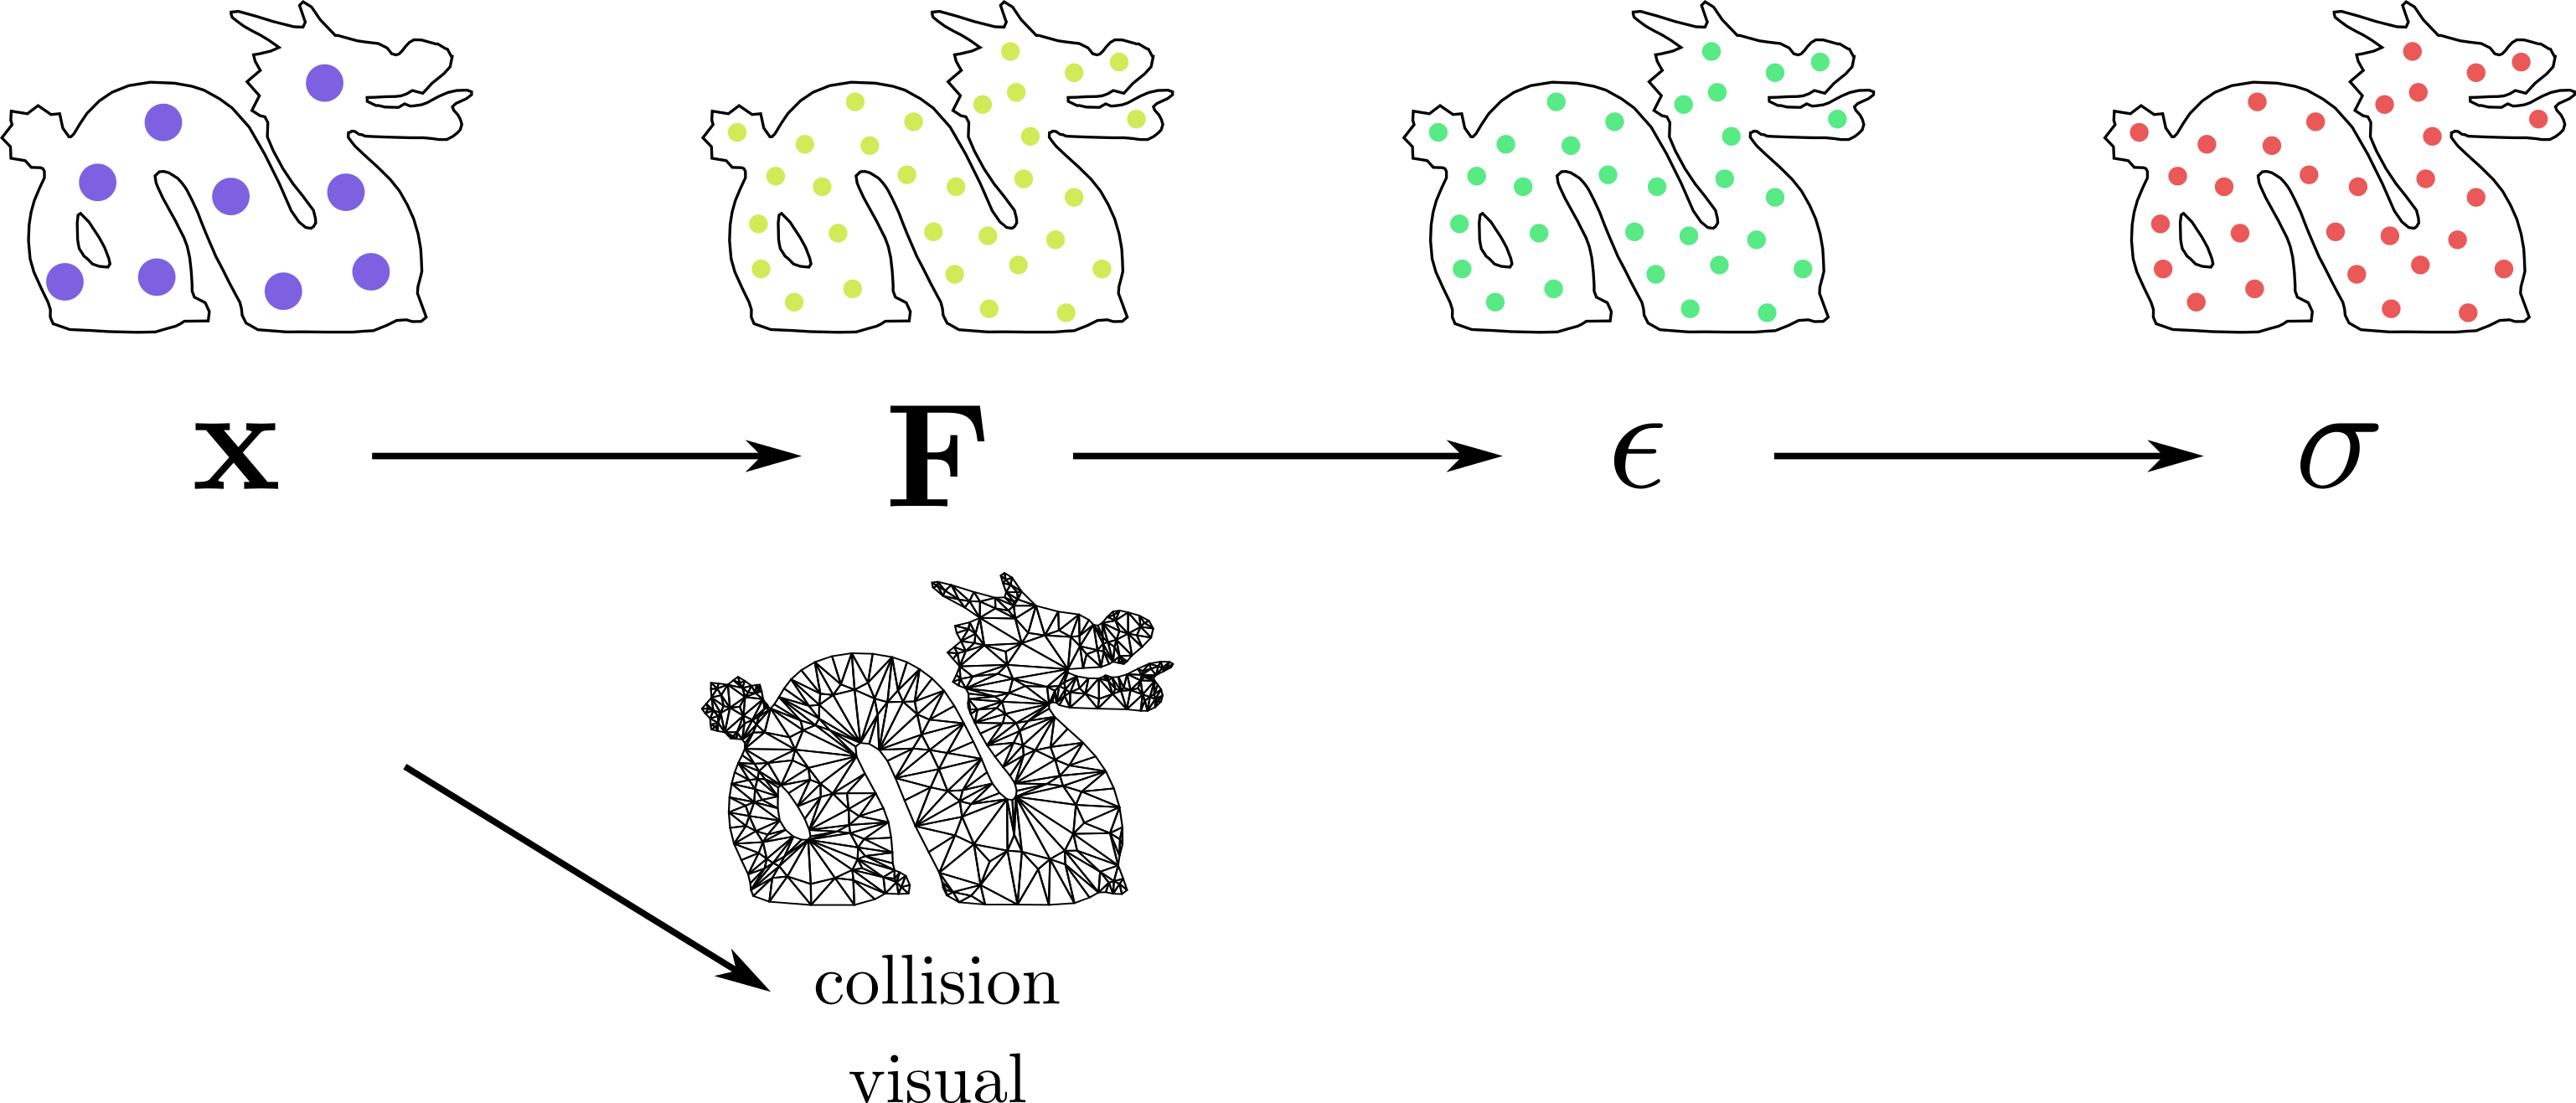
\includegraphics[scale=0.6]{./images/continuum_mechanics/multiLayeredFramework.png}
\caption[STAR mechanics: Multi-layer framework]{\label{fig:multiLayerFramework} Each component of the simulation is isolated and communicates with other components through mapping. By doing so, the framework allows fast prototyping and comparison of a wide range of deformable model.}
\end{figure}

Most of the time, the different components of a physics-based model are described as a monolithic framework: degrees of freedom, interpolation, integration and constitutive law are put together in one formula which computes the forces applied on the degrees of freedom. On one hand, this provides a compact and implentation-friendly expression. It also suits the short format of scientific article. On the other hand, it requires assumption on each component and make it hard to distinguish what should be changed in order to integrate collisions, to embed a visual model or to test variations of the initial model.

An interesting alternative is to build a multi-layer framework where each component of a physics-based model represent a layer which is able to communicate with other layers by using mappings. The framework has then a great modularity, different components can be re-used and mixed. A direct consequence is the ease at prototyping. State of the art methods can be implemented in hours instead of days. Comparison of different models is much easier. Also, it provides a way to control the granularity of a simulation. As each layer can be discretized at its own resolution, it allows for an easier repartition of resourcs and computational task.

In their work, Gilles et al. \cite{Gilles2011} proposed such an alternative by decomposing the computation of force using the derivation chain rule:
\begin{equation}
\label{eq:forceChainRule}
\mathbf{f} = -\int_{V} \left(\frac{\partial \Psi}{\partial \mathbf{x}}\right)^{T} 
=
-\int_{V} \left(\frac{\partial \mathbf{F}}{\partial \mathbf{x}}\right)^{T}
\left(\frac{\partial \epsilon}{\partial \mathbf{F}}\right)^{T}
\left(\frac{\partial \Psi}{\partial \epsilon}\right)^{T}
\end{equation}
We can now distinguish the different layers: the degrees of freedom, the deformation gradient, the strain tensor and constitutive density energy. And the the jacobian of the mapping that links degrees of freedom to deformation gradient, deformation gradient to strain and strain to constitutive density energy. Layers and mappings can be implemented separately thus providing a great deal of modularity. Moreover it is straightforward to have a sampling of degrees of freedom different from the sampling of integration points that will be used to compute deformation gradient, strain and stress.

In the case of the frame-based method, there are two additional layers, one for embedding a visual model and one for handling collisions. Both communicates with the degrees of freedom through a mapping which is the displacement field (see Figure~\ref{fig:multiLayerFramework}).

\paragraph{Degrees of freedom}
The object is uniformly sampled with affine frames as degrees of freedom. Affine frames $T=(A,t)$ represent $12$ degree of freedoms, $3$ for translation $\mathbf{t}$, $9$ for the matrix $\mathbf{A}$ combining rotation, scaling and shearing. Affine frames are represented with respect to an initial configuration ~$T_{0} = \left(A_{0}, t_{0}\right)$.

\paragraph{Interpolation}
Linear blend skinning is used to interpolate the displacement field. A deformed position $\mathbf{x}$ can be interpolated as a weighted sum of the affine transformations applied to the rest position $\mathbf{x_{0}}$.

\begin{equation}
\begin{array}{l}
\displaystyle \mathbf{x} = \sum_{i} w_{i}(\mathbf{x_{0}})\left(t_{i}+A_{i}\mathbf{x_{0}^{rel}}\right) \\
\displaystyle \mathbf{x_{0}}^{rel} = A_{0}^{-1}\left( \mathbf{x_{0}} - \mathbf{t_{0}} \right)
\end{array}
\end{equation}

where $\mathbf{x_{0}^{rel}}$ is the relative position of $x_{0}$ in the frame defined by $T_{0}$ and $w_{i}$ is the shape function associated to the frame $i$.

Different weights can be used. Three properties are important in order to represent a physical behavior. First, the shape function should linearly decrease with respect to distance in the material. Otherwise, the deformation will not be uniform with respect to the distance from the frame. Second, the shape function should be positive. Third, the weight should for a partition of unity. In practice, one can use harmonic weights or Voronoi-based weights which are described later.

From the description of the displacement field, the deformation gradient can then be derived:
\begin{equation}
\displaystyle
F\left(\mathbf{x}\right) = \sum_{i} \frac{\partial \mathbf{x}}{\partial \mathbf{x_{0}}} =
\nabla w_{i}(\mathbf{x_{0}}) \left( t_{i}+A_{i}x_{0}^{rel}\right) + 
w_{i}\left( A_{i}A_{0}^{-1} \right)
\end{equation}

\paragraph{Spatial integration}

Any quadrature rule can be used. Here, for the sake of simplicity, we suppose that we use the midpoint rule. Thus, the integral of a function $f$ over the object states:
\begin{equation}
\displaystyle
\int_{V} f(x)  = \sum_{i} V_{i} f(x_{i})
\end{equation}
where $i$ is an integration point and $V_{i}$ its associated volume.

From this quadrature rule, we can now explicit the computation of internal forces for one frame:
\begin{equation}
\label{eq:frameForceComputation}
\displaystyle
\mathbf{f}_{i} =
- \sum_{p}
\left( \frac{\partial \mathbf{F}}{\partial \mathbf{x}_{i}} \right)^{T}
\left( \frac{\partial \epsilon}{\partial \mathbf{F}} \right)^{T}
\left( \frac{\partial \Psi}{\partial \mathbf{\epsilon}} \right)^{T} \left(\mathbf{x_{p}}\right) V_{p} 
\end{equation}
where $p$ is an integration point, $\mathbf{x}_{p}$ its position and $V_{p}$ its associated volume.

\paragraph{Temporal integration}

Assuming the mass matrix is lumped and that we use explicit Euler, the time integration of one frame $i$ is:
\begin{equation}
\displaystyle
\begin{pmatrix}
t_{i}(t+\Delta t) \\
A_{i}(t+\Delta t)
\end{pmatrix} 
=
\begin{pmatrix}
t_{i}(t) \\
A_{i}(t)
\end{pmatrix} 
+
\Delta t
\mathbf{M}_{i}^{-1}
\mathbf{f}(t)
\end{equation}
where $\mathbf{M}_{i}$ is the mass matrix of the frame $i$:
\begin{equation}
\label{eq:massMatrix}
\mathbf{M}_{i} = \int_{V} \Phi_{i}^{T} \rho \Phi_{i}
\end{equation}
and $\Phi_{i}$ is the shape function of the frame $i$.

%\section[A quick \& dirty introduction to fluid dynamics]{A quick \& dirty introduction to computational fluid dynamics}
%
%\subsection{Navier-Stokes equation}
%
%\paragraph{Mass conservation}
%The conservation of mass is quite explicit. The mass of the fluid cannot change. Mathematically, it is expressed by stating that the variation of the mass in a given volume is equal to the flux of mass going through the border of the volume.
%\begin{equation}
%    \label{eq:massConservation}
%    \frac{d}{dt}\left( \int_{\mathcal{V}} \rho dx \right)
%    =
%    - \int_{\mathcal{\partial V}}\rho \mathbf{v} \mathbf{n} ds
%\end{equation}
%
%From Stokes' formula, we have
%
%\begin{equation}
%\int_{\partial \mathcal{V}} \rho \mathbf{v} \mathbf{n} ds =
%\int_{\mathcal{V}} \nabla \cdot \left( \rho \mathbf{v} \right)
%\end{equation}
%
%then the conservation of mass can be rewritten as
%
%\begin{equation}
%\int_{\mathcal{V}} \frac{d}{dt} \rho + \nabla \cdot \left( \rho  \mathbf{v} \right) dx = 0
%\end{equation}
%
%\paragraph{Constitutive Law}
%The constitutive law describes how the fluid react to a deformation. For an incompressible fluid, the fluid reacts to pressure and viscosity and can be written:
%\begin{equation}
%\sigma = -pI + \eta \left( \nabla \mathbf{v} + \nabla \mathbf{v}^{T} \right)
%\end{equation}
%
%\paragraph{Incompressibility}
%This states that the mass should not vary over time. Then the mass conservation can be rewritten as:
%\begin{equation}
%\nabla \cdot u = 0
%\end{equation}
%
%\paragraph{Momentum conservation}
%
%Also called Newton's second law, it states:
%\begin{equation}
%\label{eq:momentumConservation}
%\int_{\mathcal{V}} \rho \frac{D}{Dt} \mathbf{v}(t,x) dx = \int_{V} \mathbf{f} dx
%\end{equation}
%
%Two kind of forces are generally applied on a fluid, the \emph{external} forces and the \emph{internal} forces.
%
%External forces describe the action of the surrounding environment on the fluid, the simplest example is the gravity:
%\begin{equation}
%\int_{\mathcal{V}} \rho \mathbf{g} dx
%\end{equation}
%
%Internal forces describe the reaction of the fluid to an external deformation. A general way to describe them is by using a tensor notation:
%\begin{equation}
%\int_{\mathcal{V}} \sigma \mathbf{n} ds
%\end{equation}
%By applying the Stokes' formula we can describe it with respect to the volume:
%\begin{equation}
%\int_{\mathcal{V}} \sigma \mathbf{n} ds =
%\int_{\mathcal{V}} \nabla \cdot \sigma dx
%\end{equation}
%
%Conservation of momentum can then be rewritten:
%\begin{equation}
%\int_{\mathcal{V}} \rho \frac{D}{Dt} \mathbf{v}(t,x) dx = \int_{V} \rho \mathbf{g} + \nabla. \sigma dx
%\end{equation}
%
%Then we have:
%\begin{equation}
%\nabla \cdot \sigma = \nabla \cdot \left( -pI + \eta \left( \nabla \mathbf{v} + \nabla \mathbf{v}^{T} \right) \right) = -\nabla p + \Delta \mathbf{v}
%\end{equation}
%
%With internal forces, we have the Navier-Stokes equation for an incompressible fluid:
%
%\begin{equation}
%\begin{array}{ll}
%\int_{\mathcal{V}} \rho \frac{D}{Dt} \mathbf{v}(t,x) dx = \int_{V} \rho \mathbf{g} -\nabla p + \eta \Delta \mathbf{v} dx \\
%\nabla. \mathbf{u} = 0
%\end{array}
%\end{equation}
%
%\paragraph{Lagrangian vs Eulerian}
%
%Lagrangian: You follow the river. The river is discretized into particles which carries and update fluid properties such as position and velocity. 
%
%Eulerian : You stand in the middle of a river. The river is discretized into a fixed grid from where you can measure the velocity of the flow passing through the point of the grid.
%
%The material derivative:
%\begin{equation}
%\frac{D\mathbf{u}}{Dt} = \frac{\partial \mathbf{u}}{\partial t} + (\mathbf{u} \cdot \nabla v)
%\end{equation}
%
%In a lagrangian framework, the positions of the particles at a specific time $t$ is known, so the material derivative is just the time derivative.
%
%\begin{equation}
%\frac{D\mathbf{u}}{Dt} = \frac{\partial u}{\partial t}
%\end{equation}
%
%Moreover, if we assume that the mass of the particles is constant through the simulation, then conservation of mass is granted and we can omit its numerical solving. However, in practice it does not ensure that the divergence of the velocity will be null, new methods were proposed to enforce the null divergence condition. In this work we keep the first approximation and do not enforce the null divergence condition.
%
%\subsection{Discretization}
%
%Once equations of motion have been set, they can be discretized in space and time and integrated.
%
%\subsection{Discretization: The Smoothed Hydrodynamics Particles model}
%Smoothed Particles Hydrodynamics is an interpolation method that can be used to discretize the Navier-Stokes equation in a Lagrangian way. The fluid is discretized into particles which represent a small volume of the whole fluid and each quantity is interpolated using SPH.
%
%\paragraph{SPH interpolation}
%The interpolation of a function $f$ at a position $\mathbf{x}$ is :
%\begin{equation}
%f(\mathbf{x}) = \int_{V} f(\mathbf{x'})W(\mathbf{x}-\mathbf{x'}, h)dx'
%\end{equation}
%where $W$ is a function called \emph{kernel}. 
%
%If the fluid is discretized into particles with a mass $m$, a density $\rho$ and a volume $V$, then we can discretize the SPH interpolation as:
%\begin{equation}
%f(\mathbf{x}) = \sum_{p} f(\mathbf{x}_{p})V_{p} W(\mathbf{x}-\mathbf{x_{p}},h) = \sum_{p} f(\mathbf{x}_{p})\frac{m_{p}}{\rho_{p}} W(\mathbf{x}-\mathbf{x_{p}},h)
%\end{equation}
%
%Then derivatives can be computed and discretized the same way:
%\begin{equation}
%D^{\alpha} f(\mathbf{x}) = \int_{\mathcal{V}} f(\mathbf{x'}) D^{\alpha} W(\mathbf{x}-\mathbf{x'}, h)dx'
%\end{equation}
%
%\begin{equation}
%D^{\alpha} f(\mathbf{x})= \sum_{p} f(\mathbf{x}_{p})\frac{m_{p}}{\rho_{p}} D^{\alpha} W(\mathbf{x}-\mathbf{x_{p}},h)
%\end{equation}
%
%However, for first derivatives, the approximation does not vanish if $f$ is constant. A quick way to ensure that is to use a differentiable function $\Phi$ (in practice we use the density $\rho$) to re-write the derivative using the derivative of a product :
%\begin{equation}
%\nabla f(x) = \frac{1}{\Phi}\left(\nabla (f \Phi) - f \nabla \Phi \right)
%\end{equation}
%
%\paragraph{How to choose the kernel}
%The properties of $W$ can vary with respect to the properties of the function to be interpolated. In general, $W$ meet the following properties:
%\begin{itemize}
%\item $W$ is normalized. Thus, constants are interpolated exactly.
%\item $W$ has a compact support.
%\begin{equation}
%\parallel \mathbf{x} \parallel \geq h \rightarrow W(\mathbf{x},h) = 0 
%\end{equation}
%\begin{equation}
%\int_{\mathcal{V}} W(\mathbf{x},h) dx = 1
%\end{equation}
%\item $W$ tend to the delta function when the length scale $h$ tends to $0$.
%\begin{equation}
%\lim_{h \rightarrow 0} W(x,h) = \delta(x)
%\end{equation}
%\item $W$ should be symmetric to enforce invariance under rotation
%\begin{equation}
%W(-x,h) = W(x,h)
%\end{equation}
%\item Depending on the function to interpolate the kernel should be positive to prevent unphysical interpolated value.
%\begin{equation}
%W \geq 0
%\end{equation}
%\end{itemize}
%
%The cubic kernel from Monaghan is a good choice in practice.
%
%\paragraph{Applications to Navier-Stokes}
%
%\begin{equation}
%\rho_{i} = \sum_{j} m_{j}W(\mathbf{x_{j}}-\mathbf{x_{j}},h)
%\end{equation}
%
%\begin{equation}
%\left(\nabla p\right)_{i} = \sum_{j} \frac{m_{j}}{\rho_{j}} p_{j} \nabla W(\mathbf{x_{j}}-\mathbf{x_{j}},h)
%\end{equation}
%
%However linear and angular momentum are not conserved as the formula is not symmetric. By using the previous technique with $\Phi = \frac{1}{\rho}$, it can be symmetrized:
%
%\begin{equation}
%\left(\nabla p\right)_{i} = 
%\frac{1}{\rho_{i}}
%\sum_{j} m_{j} \left( \frac{p_{i}}{\rho_{i}^{2}} + \frac{p_{j}}{\rho_{j}^{2}} \right) \nabla W(\mathbf{x_{j}}-\mathbf{x_{j}},h)
%\end{equation}
%
%\begin{equation}
%\left(\Delta \mathbf{v}\right)_{i} = \sum_{j} \frac{m_{j}}{\rho_{j}} \mathbf{v}_{j} \Delta W(\mathbf{x_{j}}-\mathbf{x_{j}},h)
%\end{equation}
%
%Same as for the pressure gradient, this is not symmetric. Here it can be symmetrized by using $\Phi = \rho$.
%
%\begin{equation}
%\left(\Delta \mathbf{v}\right)_{i} = \frac{1}{\rho_{i}}\sum_{j} m_{j} \left( \mathbf{v}_{j}-\mathbf{v}_{i}\right) \Delta W(\mathbf{x_{j}}-\mathbf{x_{j}},h)
%\end{equation}
%
%In practice, the evaluation of the laplacian is not accurate. Another form of viscosity based on the gradient was proposed. This is still an area of research.
%
%\begin{equation}
%\left(\Delta v\right)_{i} = 
%\frac{1}{\rho_{i}}
%\sum_{j} m_{j} \Pi_{ij} \nabla W(\mathbf{x_{j}}-\mathbf{x_{j}},h)
%\end{equation}
%
%where 
%
%\begin{equation}
%\Pi_{ij} = -\frac{2hc_{s}}{\rho_{i}+\rho_{j}}\frac{v_{ij}^{T}x_{ij}}{\vert x_{ij} \vert^{2} + \epsilon h^{2}}
%\end{equation}
%
%Now if we discretize Navier-Stokes for one particle $i$, we have:
%
%\begin{equation}
%m_{i}\frac{d}{dt}v_{i}(t) = m_{i}\mathbf{g} - m_{i}(\nabla p)_{i} + m_{i}(\delta \mathbf{v})_{i}
%\end{equation}
%
%This equation can now be discretized in time and integrated. In practice we use the euler symplectic integrator:
%
%\begin{equation}
%\begin{array}{ll}
%v_{i}(t+\Delta t) = v_{i}(t) + \Delta t \frac{d}{dt}v_{i}(t) \\
%x_{i}(t+\Delta t) = x_{i}(t) + \Delta t v_{i}(t+\Delta t)
%\end{array}
%\end{equation}
%
%Several interesting implementation problems arise when dealing with particle system and more particularly particle-based fluid simulations:
%
%\begin{itemize}
%\item Boundary handling 
%\item Surface reconstruction
%\item Optimization (acceleration structure for spatial query)
%\end{itemize}
%
%Faire un tableau avec les références et ce que l'on peut y trouver d'intéressant.
%
%%\paragraph{Eulerian grid}
%%\paragraph{Lagrangian particles}
%%\paragraph{Hybrid method}
%%\paragraph{Smoothed Hydrodynamics Particles model}

%\section[A quick \& dirty introduction to continuum mechanics]{A quick \& dirty introduction to continuum mechanics}

%The behavior of an elastic deformable model is described by conservation laws and a constitutive law.
%
%The first conservation law is the conservation of mass.
%
%The second conservation law is the conservation of momentum.
%
%The constitutive law depict the behavior of the object with respect to a deformation.
%
%\begin{equation}
%\begin{array}{ll}
%\int_{\mathcal{V}} \frac{d\mathbf{v}}{dt} = \int_{\mathcal{V}} \rho \mathbf{g} + \nabla \cdot \sigma dx 
%\\
%\int_{\mathcal{V}} \nabla \cdot u = 0
%\end{array}
%\end{equation} 
%
%A common way to describe the stress tensor for elastic materials is to use a constitutive density energy:
%\begin{equation}
%\sigma = \frac{\partial \Psi}{\partial \epsilon}
%\end{equation}
%
%There are many forms of enery. For a classical Hookean material, the density energy is
%\begin{equation}
%\Psi = \frac{1}{2}H\epsilon^{2}
%\end{equation}
%
%Then the stress tensor is
%\begin{equation}
%\sigma = H\epsilon
%\end{equation}
%
%H is called the stiffness tensor and is a $3\times3\times3\times3$ tensor. For isotropic materials, the number of material parameters can be reduced to two, the Young's modulus $E$ and the Poisson's ratio $\nu$. Also, the strain and stress tensor being symmetric, the constitutive law can be simplified:
%\begin{equation}
%\sigma = 
%\begin{bmatrix}
%\sigma_{11} \\
%\sigma_{22} \\
%\sigma_{33} \\
%\sigma_{23} \\
%\sigma_{13} \\
%\sigma_{12}
%\end{bmatrix}
%=
%\tilde{H}
%\begin{bmatrix}
%\epsilon_{11} \\
%\epsilon_{22} \\
%\epsilon_{33} \\
%2\epsilon_{23} \\
%2\epsilon_{13} \\
%2\epsilon_{12}
%\end{bmatrix}
%\end{equation}
%
%where
%
%\begin{equation}
%\tilde{H} =
%\frac{E}{\left(1+\nu\right)\left(1-2\nu\right)}
%\begin{bmatrix}
%1-\nu & \nu & \nu & 0 & 0 & 0 \\ 
%\nu & 1-\nu & \nu & 0 & 0 & 0 \\
%\nu & \nu & 1-\nu & 0 & 0 & 0 \\
%0 & 0 & 0 & \frac{1-2\nu}{2} & 0 & 0 \\
%0 & 0 & 0 & 0 & \frac{1-2\nu}{2} & 0 \\
%0 & 0 & 0 & 0 & 0 & \frac{1-2\nu}{2} \\
%\end{bmatrix}
%\end{equation}
%
%The strain is used to measure the relative deformation with respect to the rest position of the object: elongation, compression. Therefore it is  linked to the variation of position of the object. In 3D, this position is described by 3 coordinates which can be derived with respect to each direction, then the strain should be represented by a $3\times3$ matrix.
%
%An object is deformed if it has been compressed, stretched or sheared. The strain should measure this deformation and be $0$ when the object is at its rest position. This constraint can be expressed as:
%\begin{equation}
%\epsilon = \left( \nabla \mathbf{x} \right)^{T} \nabla \mathbf{x} - I
%\end{equation}
%
%$\nabla \mathbf{x}$ is also called deformation gradient.
%
%For elastic object, the position is always relative to the rest position. Therefore, a displacement vector is often used to depict the current position.
%\begin{equation}
%\mathbf{x} = \mathbf{x}_{0} + \mathbf{u}
%\end{equation}
%
%Then the strain relation becomes
%\begin{equation}
%\epsilon = \nabla \mathbf{u} + \left( \nabla \mathbf{u} \right)^{T} + \left(\nabla \mathbf{u}\right)^{T}\nabla \mathbf{u}
%\end{equation}
%
%It is called the Green-Lagrange strain and its linearized version the Cauchy strain.
%
%\begin{equation}
%\epsilon = \nabla \mathbf{u} + \left( \nabla \mathbf{u} \right)^{T}
%\end{equation}
%
%The strain measurement is the big difference with respect to fluid dynamics because it is the link between the deformed object and its rest shape whereas there are no such thing when computing the stress for a fluid.
%
%Now we are ready to discretize the equations of motion in space and time.
%
%\paragraph{Discretization}
%
%Now that we have a clear description of the equation of motions, we can discretize them in space and time. Here a large number of methods can be used. 
%
%Spatial discretization are divided into two categories: mesh-based and meshfree. For both of them, different kind of degrees of freedom can be chosen. For both of them, different interpolation methods can be chosen. 
%
%Here we focus on a method called the frame-based model. The degrees of freedom are affine frames and the interpolation method is based on a method called linear blend skinning.
%
%Affine frames represent $9$ degree of freedoms, $3$ for translation, $3$ for rotation and $3$ for scaling. They uniformly sample the object and are used to compute the dynamics.
%
%For elastic objects, we need to build a mapping between the rest shape $\Omega_{0}$ and the deformed shape of the object $\Omega$ in order to compute the deformation gradient, this is called the displacement field $\Phi$.
%
%\begin{equation}
%\begin{array}{llll}
%f & \Omega_{0} & \longrightarrow & \Omega \\
%	 & \mathbf{x_{0}} & \longrightarrow & \mathbf{x}
%\end{array}
%\end{equation}
%
%In order to approximate this mapping, we use a set of functions called the shape functions $\left\lbrace \Phi \right\rbrace_{i}$. This set of functions should be consistent, i.e form a partition of unity :
%\begin{equation}
%f(\mathbf{x}) = \sum_{i} \Phi_{i}(\mathbf{x}) f(\mathbf{x}_{i})
%\end{equation}
%
%For derivatives, computation becomes straightforward:
%\begin{equation}
%D^{\alpha}f(\mathbf{x}) = \sum_{i} D^{\alpha}\Phi_{i}(\mathbf{x}) f(\mathbf{x}_{i})
%\end{equation}
%
%\begin{itemize}
%\item Collision detection and response
%\item Strain rate (viscosity)
%\end{itemize}
